% !TeX encoding = UTF-8
% !TeX spellcheck = en_US

%%
%% Copyright 2007, 2008, 2009 Elsevier Ltd
%%
%% This file is part of the 'Elsarticle Bundle'.
%% ---------------------------------------------
%%
%% It may be distributed under the conditions of the LaTeX Project Public
%% License, either version 1.2 of this license or (at your option) any
%% later version.  The latest version of this license is in
%%    http://www.latex-project.org/lppl.txt
%% and version 1.2 or later is part of all distributions of LaTeX
%% version 1999/12/01 or later.
%%
%% The list of all files belonging to the 'Elsarticle Bundle' is
%% given in the file `manifest.txt'.
%%

%% Template article for Elsevier's document class `elsarticle'
%% with numbered style bibliographic references
%% SP 2008/03/01
%%
%%
%%
%% $Id: elsarticle-template-num.tex 4 2009-10-24 08:22:58Z rishi $
%%
%%
\documentclass[preprint,12pt,3p]{elsarticle}

%% Use the option review to obtain double line spacing
%% \documentclass[preprint,review,12pt]{elsarticle}

%% Use the options 1p,twocolumn; 3p; 3p,twocolumn; 5p; or 5p,twocolumn
%% for a journal layout:
%% \documentclass[final,1p,times]{elsarticle}
%% \documentclass[final,1p,times,twocolumn]{elsarticle}
%% \documentclass[final,3p,times]{elsarticle}
%% \documentclass[final,3p,times,twocolumn]{elsarticle}
%% \documentclass[final,5p,times]{elsarticle}
%% \documentclass[final,5p,times,twocolumn]{elsarticle}

%% if you use PostScript figures in your article
%% use the graphics package for simple commands
%% \usepackage{graphics}
%% or use the graphicx package for more complicated commands
%% \usepackage{graphicx}
%% or use the epsfig package if you prefer to use the old commands
%% \usepackage{epsfig}

%% The amssymb package provides various useful mathematical symbols
\usepackage{amssymb}
\usepackage{graphicx}
\usepackage{subcaption}
\usepackage{lineno}


%% The amsthm package provides extended theorem environments
%% \usepackage{amsthm}

%% The lineno packages adds line numbers. Start line numbering with
%% \begin{linenumbers}, end it with \end{linenumbers}. Or switch it on
%% for the whole article with \linenumbers after \end{frontmatter}.
%% \usepackage{lineno}

%% natbib.sty is loaded by default. However, natbib options can be
%% provided with \biboptions{...} command. Following options are
%% valid:

%%   round  -  round parentheses are used (default)
%%   square -  square brackets are used   [option]
%%   curly  -  curly braces are used      {option}
%%   angle  -  angle brackets are used    <option>
%%   semicolon  -  multiple citations separated by semi-colon
%%   colon  - same as semicolon, an earlier confusion
%%   comma  -  separated by comma
%%   numbers-  selects numerical citations
%%   super  -  numerical citations as superscripts
%%   sort   -  sorts multiple citations according to order in ref. list
%%   sort&compress   -  like sort, but also compresses numerical citations
%%   compress - compresses without sorting
%%
%% \biboptions{comma,round}

% \biboptions{}


\journal{Automation in Construction}

\begin{document}

\begin{frontmatter}

\title{The conception of parameters and constraint-based models in architectural projects: The case of Lel\'e's pivot domes}


\author[cimatec]{Fernando Ferraz Ribeiro}
\ead{ffribeiro@gmail.com}

\author[cimatec]{Davidson Martins Moreira}
\ead{davidson.moreira@gmail.com}



\author[lcadufba]{Arivaldo Le\~ao de Amorim}
\ead{alamorim@ufba.br}

\address[cimatec]{Programa de Modelagem Computacional, SENAI Cimatec, Av. Orlando Gomes 1845, 41.650-010 Salvador, Bahia, Brazil}

\address[lcadufba]{Laborat\'orio de Computa\c{c}\~ao Gr\'afica Aplicada \`a Arquitetura e ao Desenho – LCAD, Faculdade de Arquitetura, Universidade Federal da Bahia (UFBA), Salvador, BA, Brasil}


\begin{abstract}

Following increasing interest among architects in the application of generative algorithms in the conception of projects, many questions have been raised concerning teaching this particular manner of thinking about forms. One of the main goals of learning the subject is to understand how the idea of the construction of an element can be translated into the rules of an algorithm. Other aims are to introduce the requisite programming-related concepts to implement the algorithms, and to locate this method within the scope of disciplines involved in the construction activity. This paper proposes an example-based strategy to discuss these three crucial issues by using the pivot domes designed by Brazilian architect Lel\'e as the object of study. 

\end{abstract}

\begin{keyword}
%% keywords here, in the form: keyword \sep keyword
Parametric Models \sep Geometric Constraints \sep Generative Algorithms.
%% MSC codes here, in the form: \MSC code \sep code
%% or \MSC[2008] code \sep code (2000 is the default)
\end{keyword}

\end{frontmatter}

%%
%% Start line numbering here if you want
%%
%#### numeração
%\linenumbers

%% main text
\section{Introduction}
\label{sec1}

The concepts, techniques, and applications of generative algorithms have offered significant gains in the last few decades, and have thus garnered considerable interest from architects, researchers, and teachers \cite{krish2011}. Many leading global \textit{bureaus} in the field of architecture have invested in implementing and maintaining programming departments to collaborate in the creative process of building design \cite{ceccato2010mbg}. The range of influence of computer-aided design (CAD) extrapolates the aspect of an applied tool and reaches aesthetic theories \cite{Oxman2006} \cite{picon2011} and, through integration with computer-aided manufacturing (CAM) systems, construction activities \cite{kolarevic2003}. Generative algorithms have contributed to this process.

In the academic world, the assimilation of the methods, tools, and knowledge involved in the understanding of generative design paradigms presents a range of possibilities and opportunities to rethink relations among disciplines involved in the design activities \cite{kolarevic2003} \cite{aag2010113}.

One of the main issues in teaching generative design to novice users is to make them understand how an initial idea can be translated into rules that generate forms. Understanding how these forms can be generated is the first step in this different approach to project activities encouraged by such algorithms. It is important to remember that this generation of forms in not an objective in itself, but merely a tool to assist in answering questions raised by architecture as an interdisciplinary domain. In that sense, the building of effective generative algorithms also relies on understanding the characteristics of the building or construction element that may need to be explored and tested by the process, and the manner in which different parameters act together in a way that the variety of forms created by them establish a set of possible solutions, each one with particular characteristics, to be disposed of or adopted by the user.

This paper proposes an example-based strategy to introduce generative algorithms to students through the definition of the rules that governs a conceptual parametric model of an architectural element based on parameters and constraints. The geometrical constructions used, the concepts concerning list manipulation-based programming, and aesthetics aspects of the generated forms are presented and discussed from an interdisciplinary perspective.

Although aimed at architecture and construction, the contents explored in this article can be easily adopted by oder fields, such as mechanical engineering, robotics, product design, among others. Whenever a demand exists for the conception of a form to be built, and the variations of this form could generate gains or losses in some performances or characteristics of the final product, the parametric design strategies could collaborate in obtaining better results within the same period. 


\section{Generative design and generative algorithms}
\label{generaalgor}

Algorithms are defined as a finite set of rules that describe steps to solve a specific problem \cite{knuth1997art}. The technical drawings applied in the design of architectural plans are, indeed, algorithms \cite[chap. 3]{terzidis2006algorithmic}, and the sequential operations with compass, rule, and straight edges that are used to make geometrical constructions describe the relevant rules. Words such as "perpendicular," "parallel," and "tangent" summarize entire algorithms in the drafter's vocabulary. The development of CAD technology, began by providing the ability to reproduce drawing algorithms through software, and have since evolved to a "wider graphic vocabulary available to designers, together with a more elaborate syntax---in all, a richer and potentially more expressive graphic and spatial language" \cite[chap. 15]{mitchell2008}.

\begin{figure}[!h]
\begin{center}
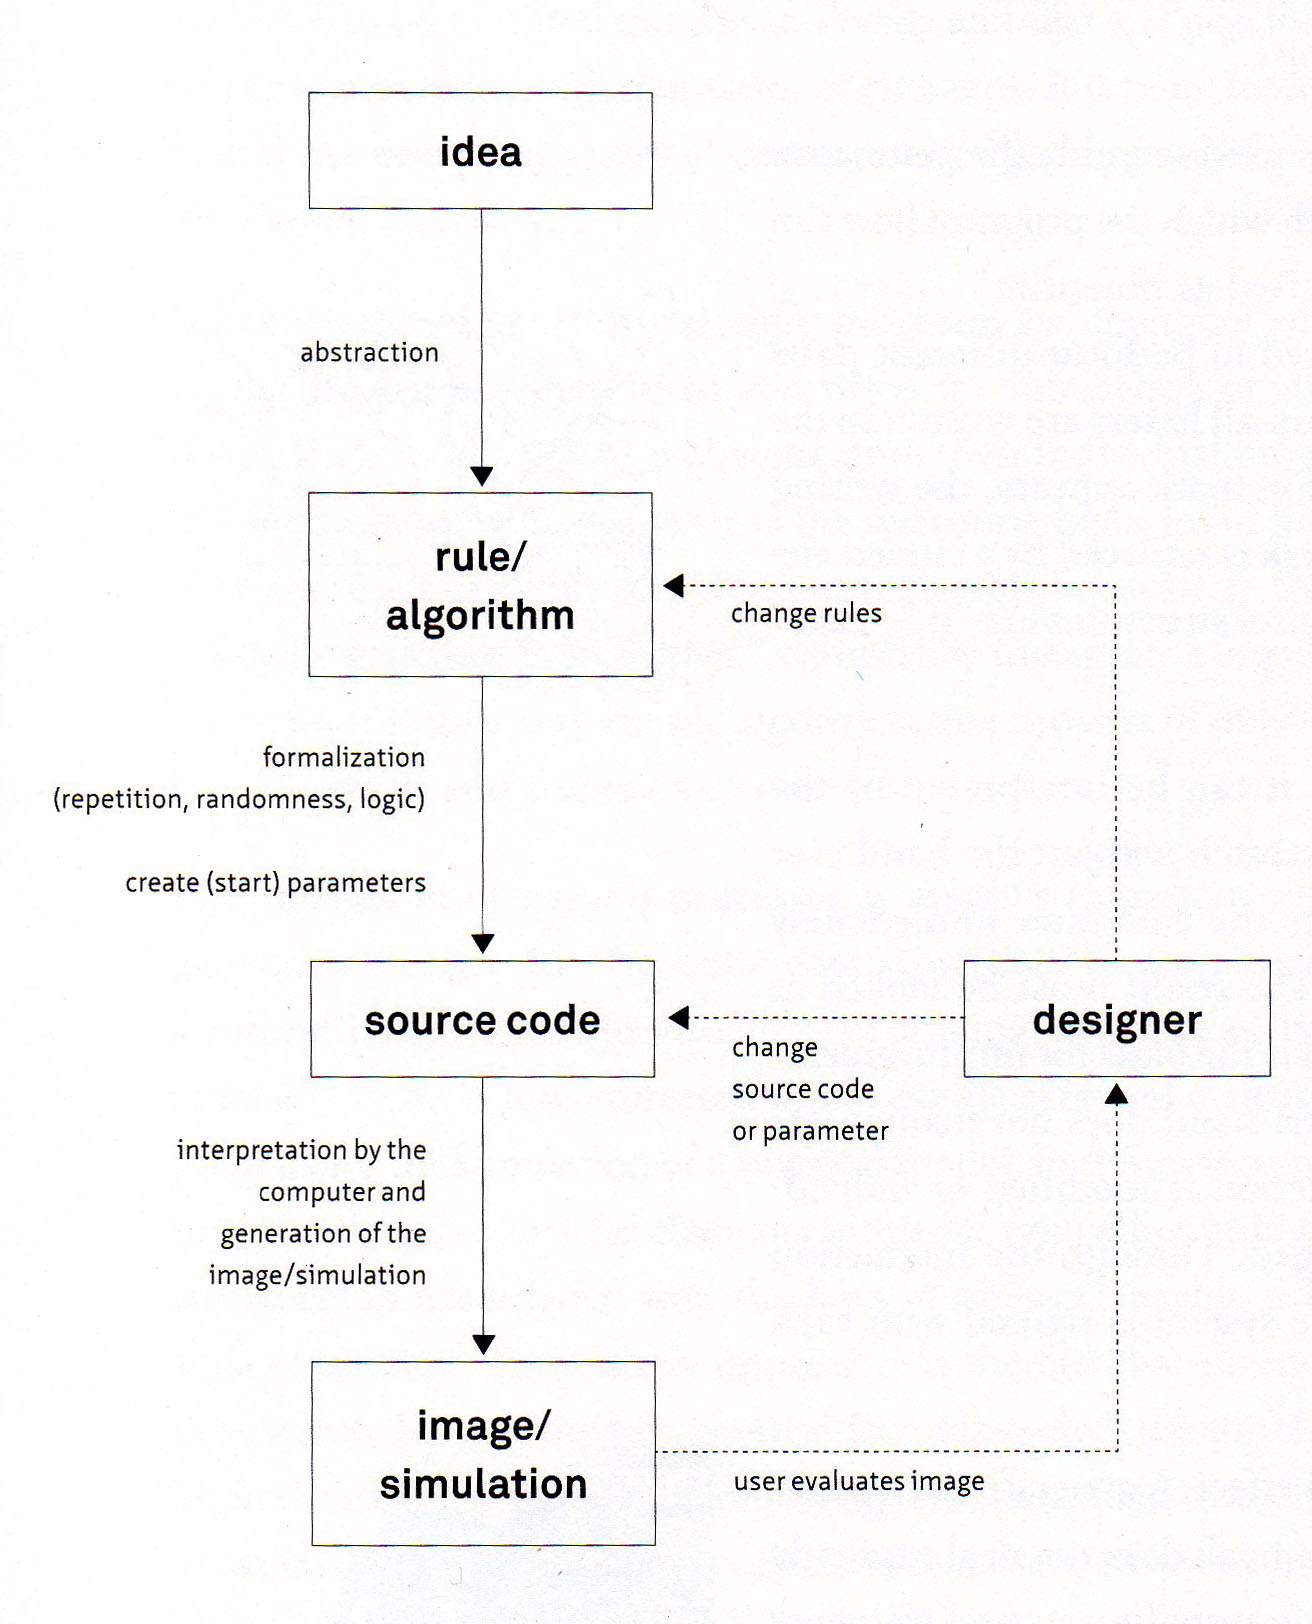
\includegraphics[width=0.5\textwidth]{fluxogramametodologia.jpg}
\caption{Flowchart of a generative algorithm}
\label{figura:fluxogramametodologia}
\end{center}
\end{figure}

Generative design can broadly be defined as the application of algorithms or a "rule-based process through which various potential design solutions can be created" \cite{fasoulaki2008}. Generative algorithms are the core engine propelling this design strategy in the computational context. As stated above, all technical drawings in constructions are algorithms of a sort. The variety of buildings designed using these methods is innumerable. Generative design techniques differ from traditional methods for transforming the methodology of work. Generative systems lend a degree of automaticity to the process, hence enabling the user to evaluate a greater number of possible solutions to the architectural problem in a shorter amount of time than would be possible through traditional methods.


In Fig. \ref{figura:fluxogramametodologia} \cite{bohnacker2012}, a flowchart illustrates the proceedings for creating and operating a generative algorithm. The real shift promoted by generative algorithms is in the process of electing the form to be constructed. It starts with an idea of what the constructed object should be, as an abstraction that is translated into a set of rules. An algorithm is implemented in a programming language, code, or a visual programmable ambiance. A simulation of the model is generated by setting parameters values and executing the algorithm. The designer evaluates the output and, by changing the parameters values, the rules, and/or the code, generates different outputs and chooses the final solution among these. The construable artifact appears only when the designer elects the proposal to be built \cite{DIno2012}.

Many computational methods have been applied for the creation of forms driven by generative algorithms: shape grammars \cite{stiny1972} \cite{Stiny1978} \cite{duarte2005} \cite{tepavcevic2012}, genetic algorithms \cite{caldas1999} \cite{fasoulaki2008} \cite{Troiano2012} \cite{Caldas2002}, cellular automata  \cite{Herr2007}, simulated annealing \cite{Ceranic2001} \cite{Correia2001} \cite{Lamberti2008}, tabu search \cite{Bland1991}, swarm intelligence \cite{Luh2011} \cite{Yahya2014}, and parametric models \cite{Turrin2011} \cite{Fischer2005} \cite{lachauer2011a} \cite{Milena2010a}, among others.

\section{Parameter- and constraint-based models (PCM)}
\label{ParamConst}

All generative algorithms, as well as all computer processing, are based on parameters, although their parametric design differs from those of others due to its emphasis on the manipulation of parameters \cite{DIno2012}. To draw a right prism in a CAD system, the user needs to enter values for width, height, and depth. In a parametric design system, each of these inputs can be interactively modified, and the dimensions of the prism are automatically updated in the drawing.

Among the many simulation methods to implement a generative design system, the Constraint Solver, since its introduction by Pro/Engineer in the 1980s, was adopted by most CAD systems \cite{Hoffmann2005}. It has garnered considerable research interest due to its intuitive and fluid manipulation of forms. The method relies on the satisfaction of constraint problems that, given a finite set of variables, consist of the assignment of these to a finite domain such that the values taken together are restricted by certain constraints, and finding a combination of these values that satisfies all constraints \cite{Bartk01theoryand}. The definition of parameter- and constraint-based models proposed here is a way of emphasizing both the parameters and the constraints that define a generative design process. 

The creation and manipulation of geometric forms in an ambiance that enables the use of a constraint solver is closely related to proof theory for geometric theorems \cite{Hoffmann2005}. Geometry has been a cornerstone of architecture and construction throughout history \cite{ceccato2010mbg}, and the teaching of generative algorithms should explore geometrical knowledge from an alternative point of view.  

\section{Object of study}
\label{obstudy}

The Brazilian architect Jo\~ao Filgueiras Lima, better known by his nickname Lel\'e, is one of the most important and celebrated architects of the country \cite{ARQ:359533}. He is considered by Oscar Niemeyer to be a "great master of architecture," and by Lucio Costa as "the architect in whom art and technology meet and merge" \cite{ferraz2000joão}. His works reveal a strong interest in rational use of materials, an outstanding development of prefabrication and environmental integration, and adopting innovative daylight and air circulation solutions \cite{Campagnol2014} \cite{Maciel2007}.

\begin{figure}[!h]
\begin{center}
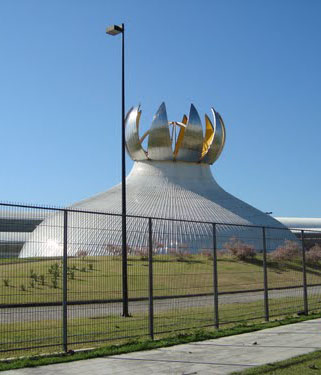
\includegraphics[width=0.3
\textwidth]{sarahcupula.jpg}
\caption{Sarah Kubitschek Hospital auditorium, Rio de Janeiro - RJ  -  www.sarah.br}
\label{figura:sarah}
\end{center}
\end{figure}

As an object of study, we used the pivoting domes in the auditorium of the Sarah Kubitschek Hospital in Rio de Janeiro (Fig. \ref{figura:sarah}), and in two buildings of the Labor Justice Courthouse complex in the city of Salvador. Figure \ref{figura:trt} shows a 3D model of the complex, with the dome of the auditorium to the right and that of the main court to the left.


\begin{figure}
\begin{center}
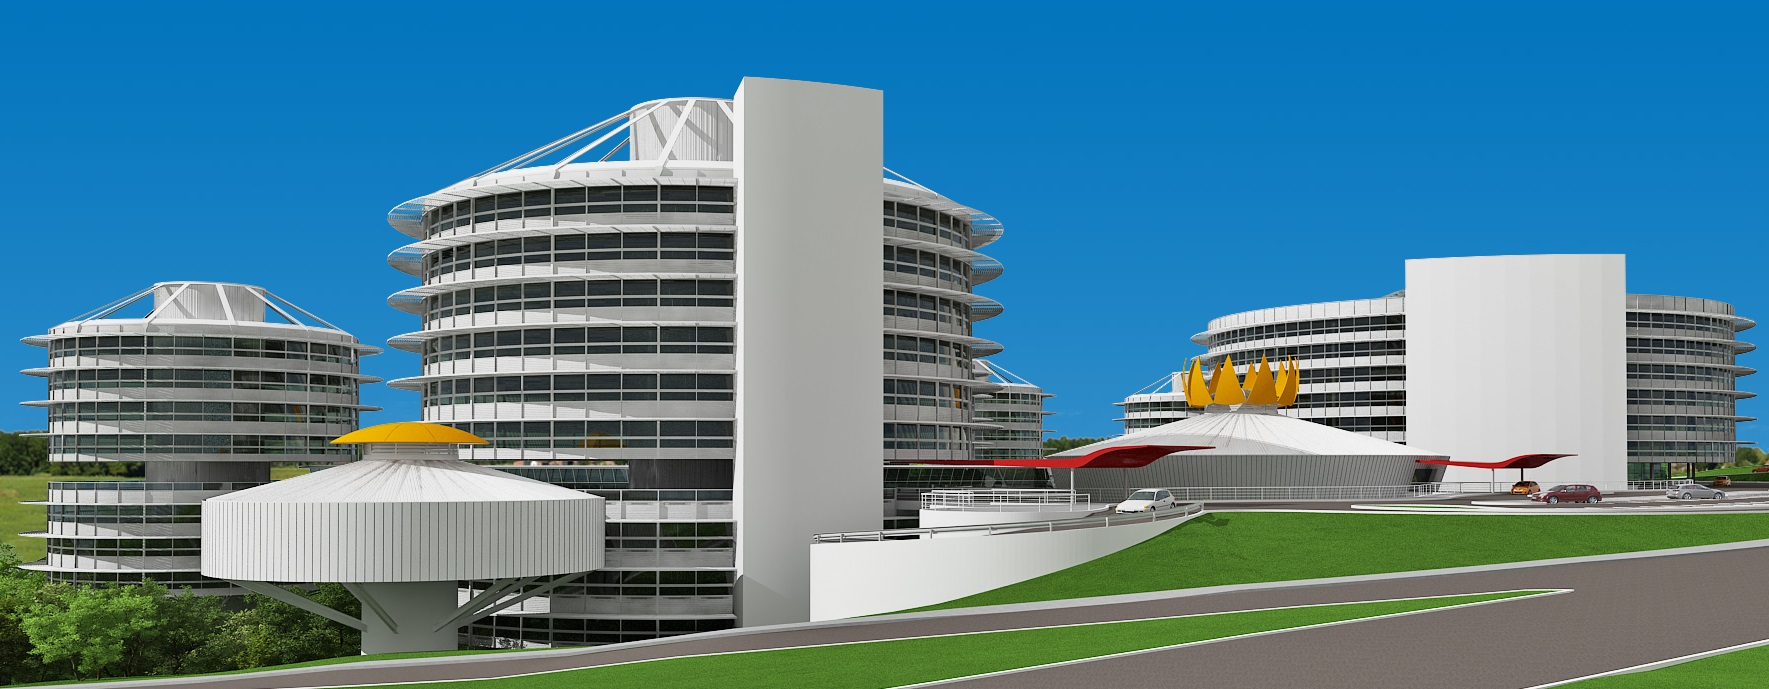
\includegraphics[width=0.7
\textwidth]{trt.jpg}
\caption{Labor Justice Courthouse Complex, Salvador - Ba. Source: Instituto Habitat archives}
\label{figura:trt}
\end{center}
\end{figure}

The first box in the flowchart in Figure \ref{figura:fluxogramametodologia} represents the idea of the family of forms to be generated. There are didactic advantages to presenting image references to illustrate the idea underlying the generative algorithms to be built. Instead of describing the abstract idea of a goal, the architectural examples clarify important aspects of the intended solution. The application of these elements to real projects, the aesthetic composition that emerged from the varying forms of the domes and their relation with the of which buildings they are part, and the fact that many aspects of the algorithm can be visually identified in the processes, can be mentioned as exemplars. A discussion of a one-sentence definition of the underlying idea could be conducted in class, or one such sentence could be proposed by the teacher to motivate discussion. The summarized idea should point students' attention to the goals of the algorithm being studied. "A dome, divided into petals that pivot around axes on their base" is a good example of a definition of the idea.


\section{Defining the parameters}
\label{implem}

Starting from the idea, the pivoting domes shown in Figures \ref{figura:sarah} and \ref{figura:trt} should be translated into algorithms that can automatically draw variations of these forms. Analyzing the domes in Figures \ref{figura:sarah} and \ref{figura:trt}, the similarities and differences between the chosen solutions can be listed:

\begin{itemize}
\item All domes are, when closed, spherical caps.
\item There are varying numbers of petals in the examples.
\item The base radii and heights of the spherical caps in the examples are different.
\item The bases of the petals are at the bases of the spherical caps.
\item The tops of the petals are at the maximum height of the sphere.
\end{itemize}

Based on this visual observations, many elements of the algorithm can be defined. The parameters, for instance, can be the base radius, the center of the base, the maximum height, and the number of petals. Another parameter should be added to the algorithm to simulate the pivoting movement of the dome: a rotation angle parameter.

It is important to note that other parameters can replace the selected ones to draw the same forms. The radius of the full sphere and the differences between the cap height, the center of the sphere, and the sphere radius, for example, can replace the maximum height, the base center, and the cap base radius generating the same geometries. Although equivalent results can be accomplished by the proposed strategies, it is good practice to think about the characteristics of the construction element that are intended to be explored, and how the parameters to be manipulated fit into the process. Let us assume that in the example, the main characteristics to be explored are the area of illumination and ventilation provided by the dome when open, and the aesthetic relationship between the radius and the maximum height. This assumption justifies the proposed parameters, as they directly affect the characteristics under consideration.


\section{Geometric constructions and constraints}
\label{geometric}

\begin{figure}
\begin{subfigure}{0.3\textwidth}
  \centering
  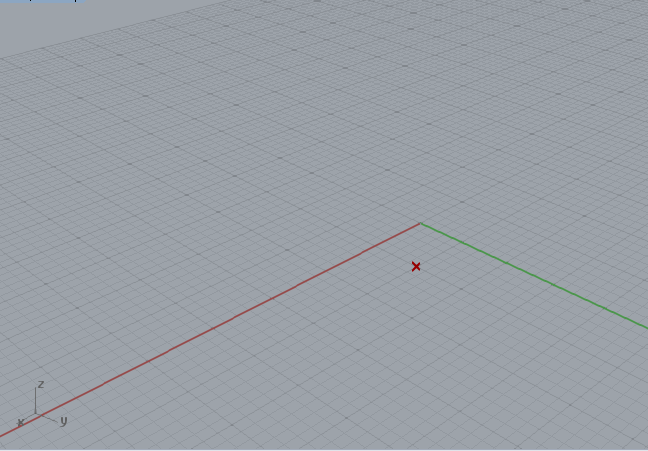
\includegraphics[width=.9\linewidth]{a01s00.png}
  \caption{Initial point}
  \label{fig:a01s00}
\end{subfigure}%
\begin{subfigure}{0.3\textwidth}
  \centering
  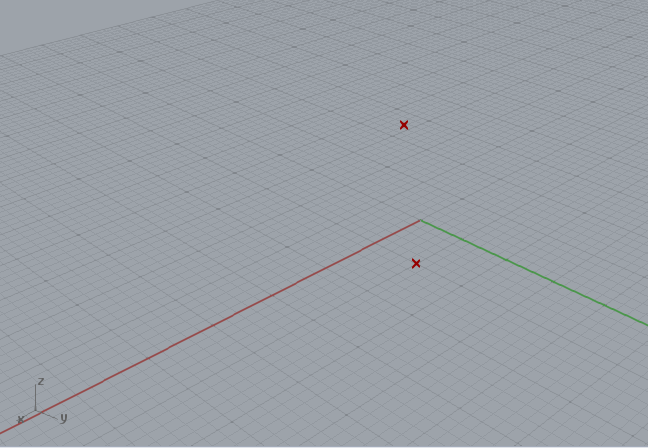
\includegraphics[width=.9\linewidth]{a01s01.png}
  \caption{Height point}
  \label{fig:a01s01}
\end{subfigure}
\begin{subfigure}{0.3\textwidth}
  \centering
  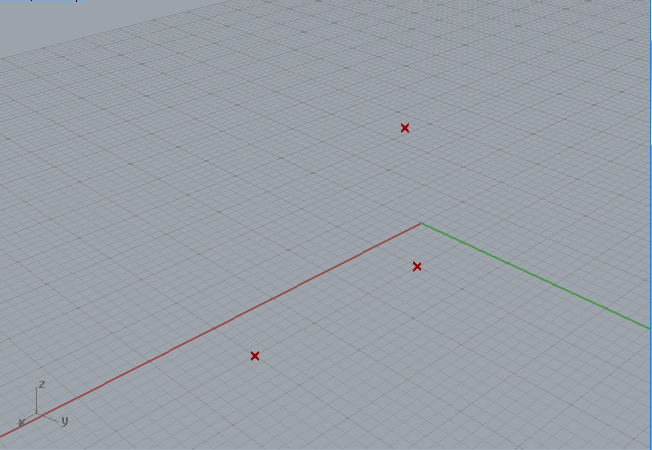
\includegraphics[width=.9\linewidth]{a01s02.png}
  \caption{Point on the base}
  \label{fig:a01s02}
\end{subfigure}


\begin{subfigure}{0.3\textwidth}
  \centering
  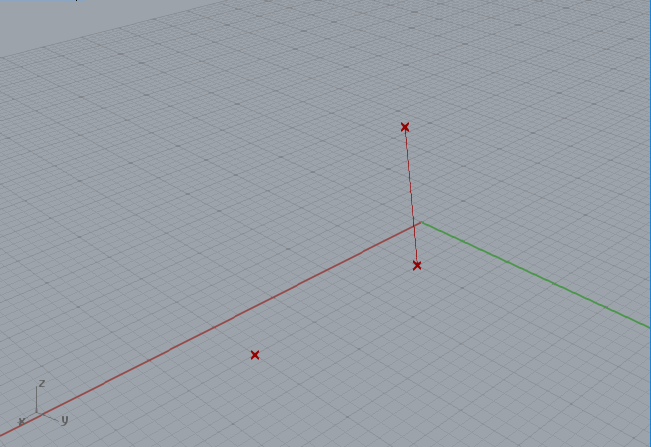
\includegraphics[width=.9\linewidth]{a01s03.png}
  \caption{Dome axis}
  \label{fig:a01s03}
\end{subfigure}
\begin{subfigure}{0.3\textwidth}
  \centering
  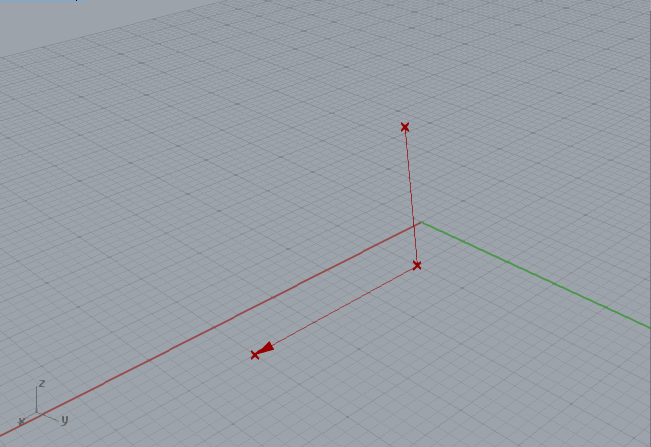
\includegraphics[width=.9\linewidth]{a01s04a.png}
  \caption{Auxiliary vector}
  \label{fig:a01s04a}
\end{subfigure}
\begin{subfigure}{0.3\textwidth}
  \centering
  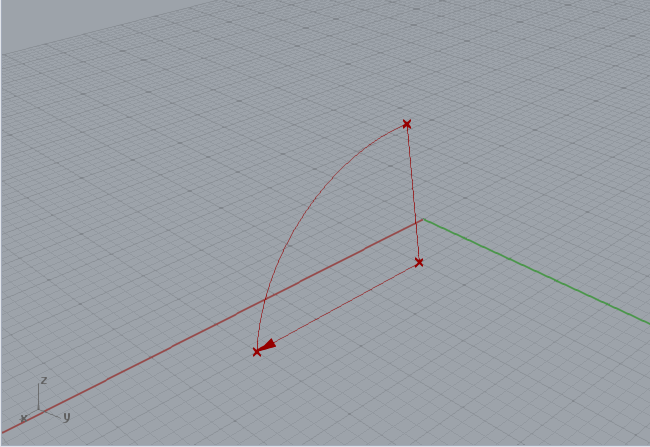
\includegraphics[width=.9\linewidth]{a01s04b.png}
  \caption{Petal arch}
  \label{fig:a01s04b}
\end{subfigure}


\begin{subfigure}{0.3\textwidth}
  \centering
  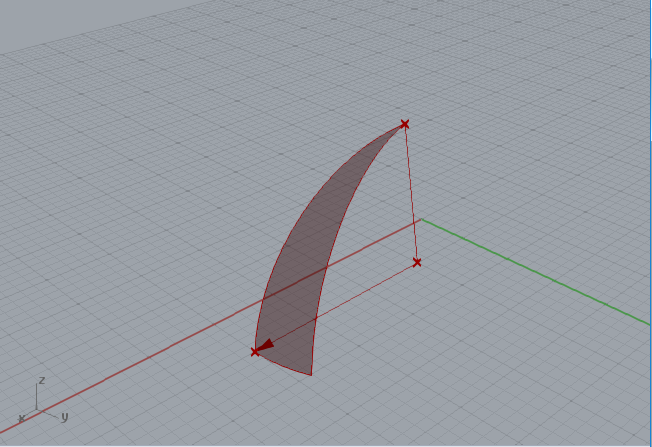
\includegraphics[width=.9\linewidth]{a01s06.png}
  \caption{Petal surface}
  \label{fig:a01s06}
\end{subfigure}
\begin{subfigure}{0.3\textwidth}
  \centering
  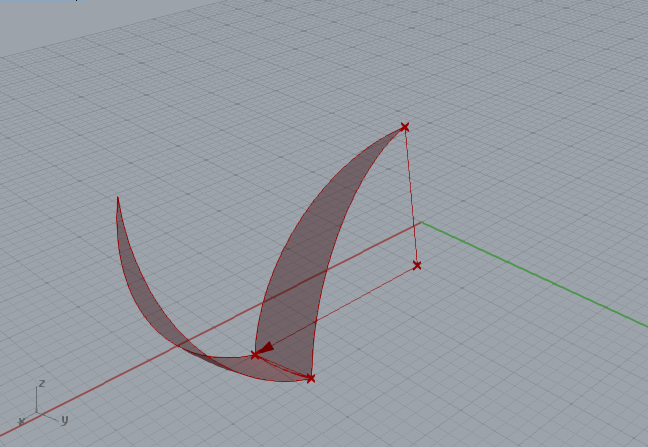
\includegraphics[width=.9\linewidth]{a01s08.png}
  \caption{Rotated petal}
  \label{fig:a01s08}
\end{subfigure}
\begin{subfigure}{0.3\textwidth}
  \centering
  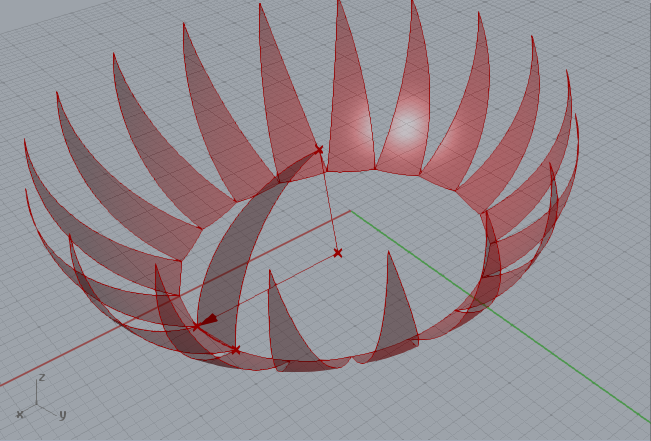
\includegraphics[width=.9\linewidth]{a01s09.png}
  \caption{Full dome}
  \label{fig:a01s09}
\end{subfigure}


\caption{Steps of the one-petal algorithm}
\label{fig:a01steps}
\end{figure}

In the environment of a geometric constraint solver, the definition of the rules (constraints) can only be conceived by planning the geometric constructions. The first modeling strategy presented in this paper is to model one petal, define a rotation axis (associated with the rotation angle parameter), and copy it around a circle. Figure \ref{fig:a01steps} shows the steps of the algorithm, which are discussed below.

Starting from the \textbf{center} (Fig. \ref{fig:a01s00}) of the base circle, we make two copies of the point: one along the $z$-axis, by the distance entered as the cap height parameter, called the \textbf{height point} (Fig. \ref{fig:a01s01}), and the other along the $x$-axis, taking the value of the base radius as the module of the translation vector, referred to as a \textbf{point on the base} (Fig. \ref{fig:a01s02}). A line between the \textbf{base center} and the \textbf{height point} is also drawn, and is called the \textbf{dome axis} (Fig. \ref{fig:a01s03}).

The next step is drawing the arc on one side of the petal. As the arcs are drawn independently, the rules that define them should constrain the closed dome as a spherical cap. One of the ways to effectively constrain this construction is to make the arc be a tangent, at the height point, to a line or vector parallel to a line drawn from the base center to the point on the base. Figure \ref{figura:tangente}, illustrates this idea by showing that only the blue arcs, which are tangent to the green vectors at the height point, together form a circle arch.


\begin{figure}[!h]
\begin{center}
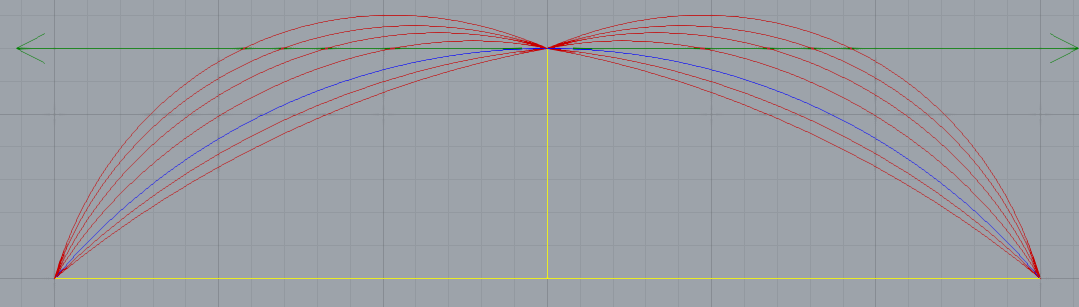
\includegraphics[width=0.65
\textwidth]{tangentes.png}
\caption{Constraining the arcs as part of a spherical cap}
\label{figura:tangente}
\end{center}
\end{figure}

In this step of the algorithm, an opportunity to debate some aspects of the geometric constructions applied in the process should be noted. More precisely, we can reflect on how this arc is defined in classical geometrical drawings, and how this construction is translated into the computational environment. 

\begin{figure}[!h]
\begin{center}
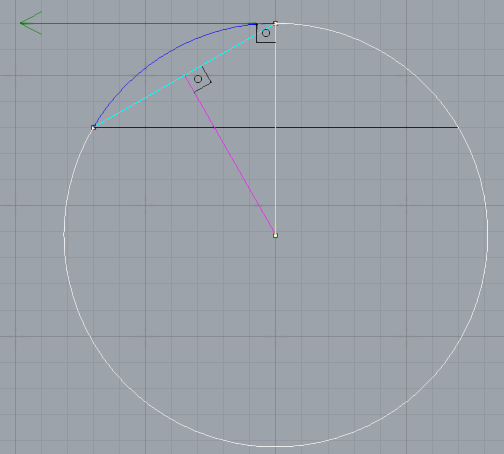
\includegraphics[width=0.5
\textwidth]{classicalarch.png}
\caption{The traditional method to draw a tangent arc}
\label{figura:classicalarch}
\end{center}
\end{figure}

The traditional steps to draw a tangent arc are shown in Figure \ref{figura:classicalarch}. The construction is based on two properties of circular arcs. One is that the tangent at every point is perpendicular to the radius at the same point. The other is the most basic property of a circle---that every point on it is equidistant to the center.

By starting with the two red points and the tangent vector, represented by the green line in Figure \ref{figura:classicalarch}, and drawing a line perpendicular to the vector at the point where the vector is tangent to the arc, it is safe to say that this perpendicular line (yellow) intersects the center of the sphere. The next step is to find a point on the perpendicular line equidistant to the two points of the arc. This can be done by drawing a segment that connects the two points (cyan), and a perpendicular line through the middle (magenta). The point of intersection of the line perpendicular to the tangent vector and the line drawn through the midpoint of the line connecting the two known points of the arc is equidistant (as are the sides of an isosceles triangle) to these points. Hence, with a compass centered on this intersection, and starting from one of the known points to the other, the arc can be defined (blue).

\begin{figure}[!h]
\begin{center}
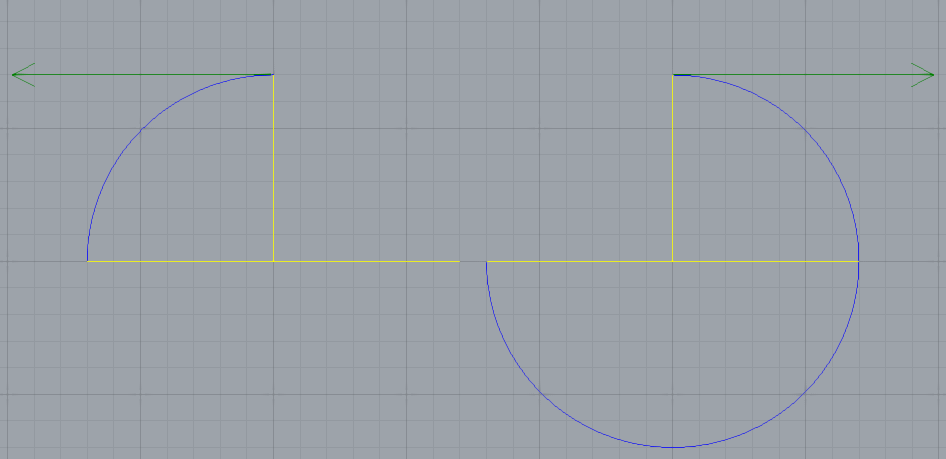
\includegraphics[width=0.5
\textwidth]{computationalarch.png}
\caption{The computational method for drawing the tangent arc}
\label{figura:computationalarch}
\end{center}
\end{figure}

Is important to note that the white arc in Figure \ref{figura:classicalarch} is also tangent to the vector, and contains the two known points. The decision to draw one arc or the other, in the traditional method, is made manually, and relies on an understanding of the intended construction. An arc perpendicular to a line is drawn by considering the orientation of the line but not its sense. In the computational environment, when this method of drawing an arc based on two points and a line is implemented, the sense of the line is used to define the sense in which the arc should be drawn. Figure \ref{figura:computationalarch} shows the arcs generated by the method using vectors with opposite senses.

In the proposed algorithm, the reference vector is defined by an ordinate segment from the \textbf{base center} to the \textbf{point on the base} (Fig. \ref{fig:a01s04a}). The command that generates an arc from two points and a vector has, as inputs, the \textbf{height point}, the \textbf{point on the base}, and the vector of the tangent to the \textbf{height point} (Fig. \ref{fig:a01s04b}). Constructing the arc in this manner constrains the closed dome to a spherical cap, with the height and base radius assuming the values defined by the respective parameters.

The petal is created as a ruled surface, generated by a rotation around the \textbf{dome axis} in an angle called the \textbf{petal angle} (Fig. \ref{fig:a01s06}). It is obtained by dividing a $360 ^{\circ}$ angel ($2 \times \pi $ in radians) by the \textbf{number of petals}. 

To simulate the pivoting movement that opens the dome, a rotation axis connecting the base points of the petal needs to be created. This can be done by rotating the \textbf{point on the base} around the \textbf{dome axis} by taking the \textbf{petal angle} as the extent of rotation. A line is drawn between the two points, and is called the \textbf{pivot axis}.

The petal surface is rotated around the \textbf{pivot axis} by an angle defined by the \textbf{pivot rotation} parameter (Fig. \ref{fig:a01s08}). To complete the algorithm and generate the \textbf{full dome} (Fig. \ref{fig:a01s09}), a polar array of the \textbf{rotated petals} is generated in a $360 ^{\circ}$ angle around the \textbf{dome axis} by taking the number of petals as the number of elements of the array.

\section{The code}
\label{code}

Although virtually any programming language can be used to implement the code, the CAD software Rhinoceros 3D (version 5.11) and its plug-in Grasshopper (version 0.9.0076) were chosen due to the intuitive nature of programming through the connection of graphical components, as well as the fact that the forms would hence be created inside a CAD system that can accommodate architectural projects.

\begin{figure}[!h]
\begin{center}
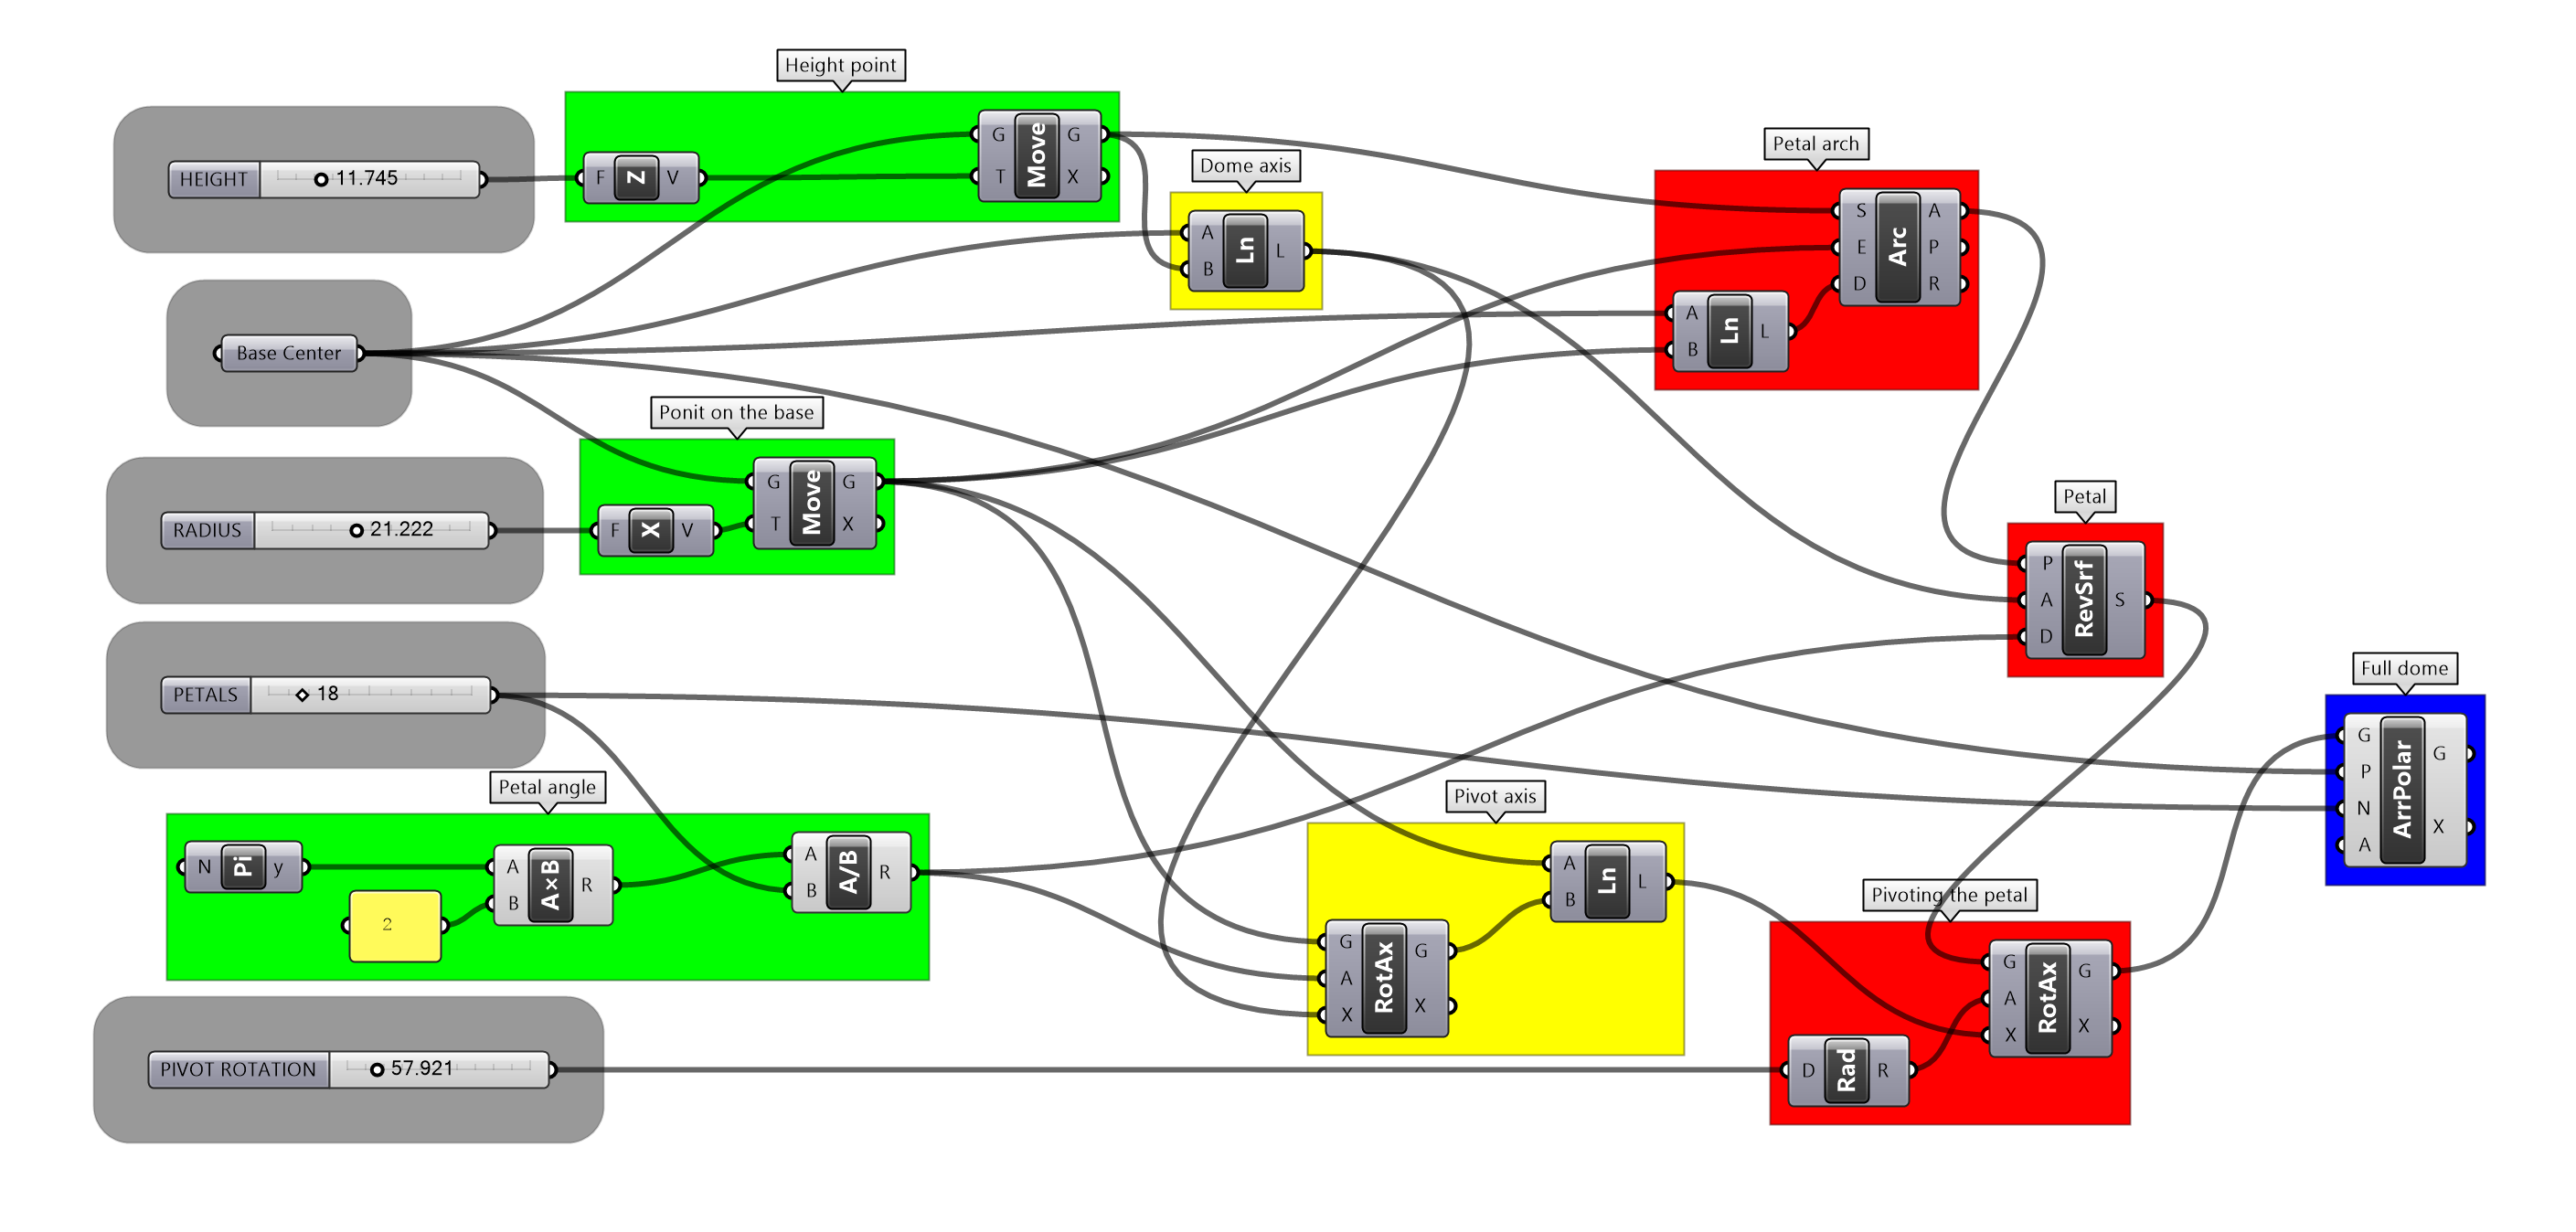
\includegraphics[width=0.95
\textwidth]{alg01.png}
\caption{One-petal algorithm}
\label{figura:alg01}
\end{center}
\end{figure}

Figure \ref{figura:alg01} shows the code implemented on the programming interface as well as a flowchart of the algorithm. Data flows from left to right through wire-like connections between components.

The grey boxes show the parameters. From top to bottom: \textbf{height}, \textbf{base center}, \textbf{radius}, \textbf{number of petals}, and \textbf{pivot rotation}. The top green box generates the \textbf{height point}, the middle green \textbf{the point on the base}, the bottom green calculates the \textbf{petal angle}. The yellow box on top generates the \textbf{dome axis} by taking the \textbf{base center} and the \textbf{height point} as inputs, and the bottom yellow generates the \textbf{pivot axis}. The \textbf{auxiliary vector} and the \textbf{petal arch} are calculated in the top red box, the middle red box performs the revolutions that generated the \textbf{petal surface}, and the bottom red box rotates it around the \textbf{pivot axis}. The blue box is responsible for the polar array operation that generates the \textbf{full dome}.



\section{List manipulation-based algorithm}
\label{listmanip}

\begin{figure}
\begin{subfigure}{0.3\textwidth}
  \centering
  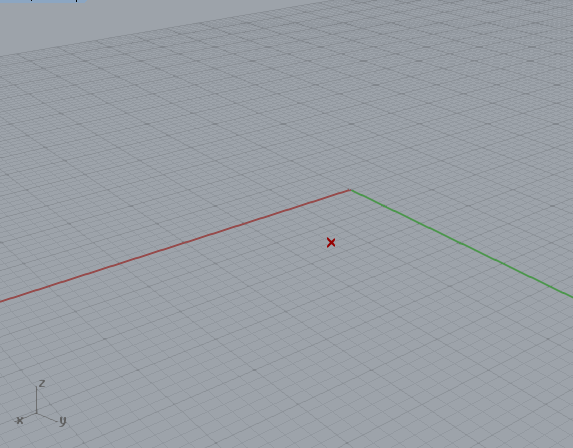
\includegraphics[width=.9\linewidth]{a02s00.png}
  \caption{Initial point}
  \label{fig:a02s01}
\end{subfigure}%
\begin{subfigure}{0.3\textwidth}
  \centering
  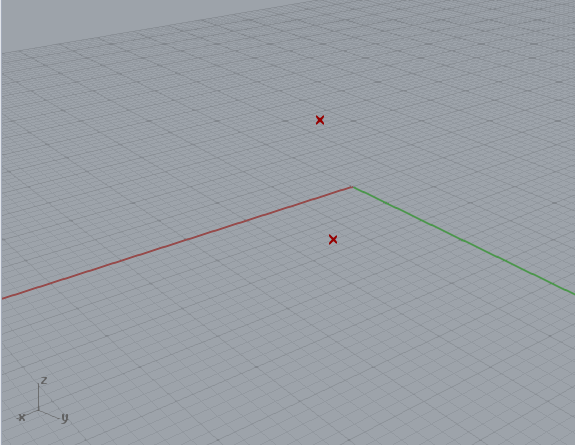
\includegraphics[width=.9\linewidth]{a02s01.png}
  \caption{Height point}
  \label{fig:a02s02}
\end{subfigure}
\begin{subfigure}{0.3\textwidth}
  \centering
  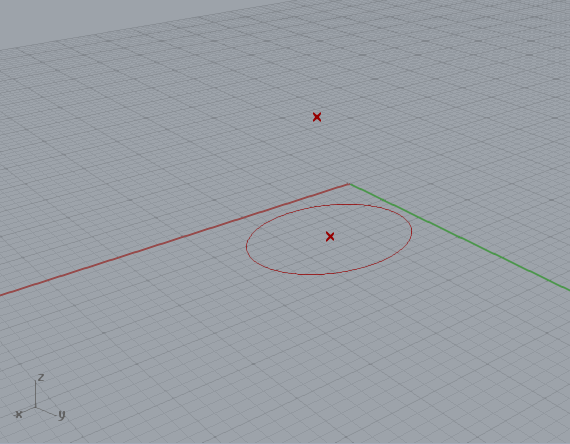
\includegraphics[width=.9\linewidth]{a02s03.png}
  \caption{Base circle}
  \label{fig:a02s03}
\end{subfigure}


\begin{subfigure}{0.3\textwidth}
  \centering
  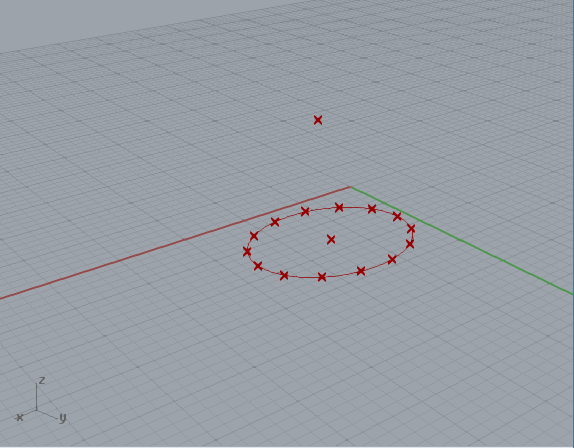
\includegraphics[width=.9\linewidth]{a02s04.png}
  \caption{Base points list}
  \label{fig:a02s04}
\end{subfigure}
\begin{subfigure}{0.3\textwidth}
  \centering
  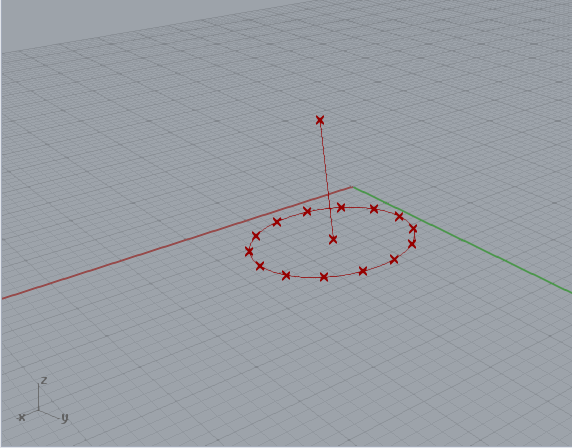
\includegraphics[width=.9\linewidth]{a02s05.png}
  \caption{Dome axis}
  \label{fig:a02s05}
\end{subfigure}
\begin{subfigure}{0.3\textwidth}
  \centering
  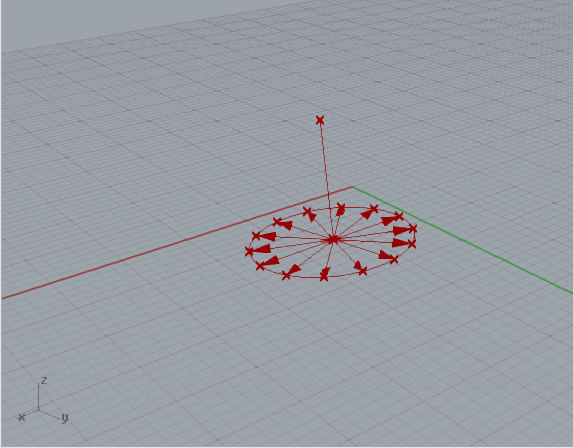
\includegraphics[width=.9\linewidth]{a02s06.png}
  \caption{Auxiliary vectors list}
  \label{fig:a02s06}
\end{subfigure}


\begin{subfigure}{0.3\textwidth}
  \centering
  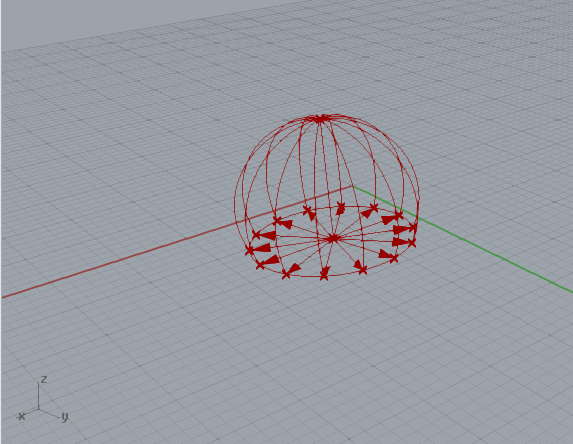
\includegraphics[width=.9\linewidth]{a02s07.png}
  \caption{Petals arcs list}
  \label{fig:a02s07}
\end{subfigure}
\begin{subfigure}{0.3\textwidth}
  \centering
  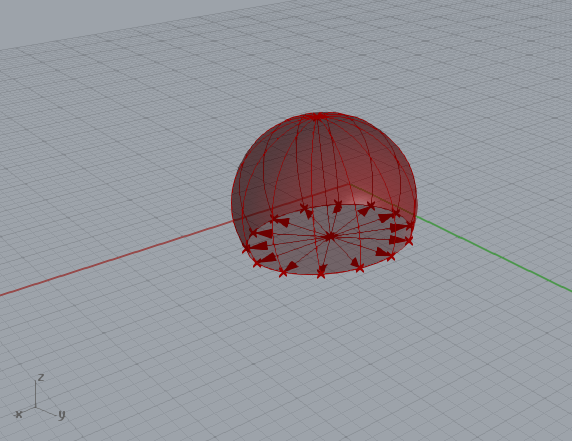
\includegraphics[width=.9\linewidth]{a02s08.png}
  \caption{Petals surfaces list}
  \label{fig:a02s08}
\end{subfigure}
\begin{subfigure}{0.3\textwidth}
  \centering
  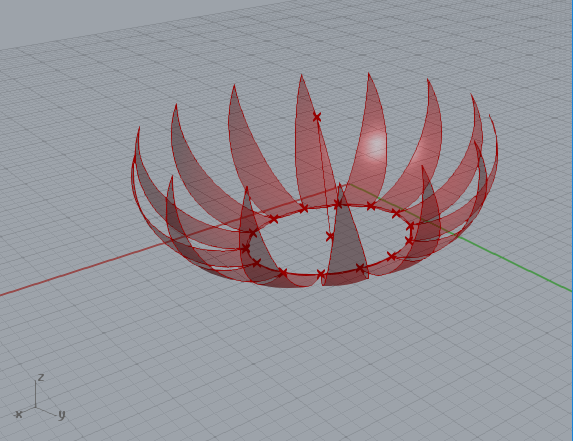
\includegraphics[width=.9\linewidth]{a02s09.png}
  \caption{Full dome}
  \label{fig:a02s09}
\end{subfigure}


\caption{Steps of the list manipulation-based algorithm}
\label{fig:a02steps}
\end{figure}

The one-petal algorithm presented in the preceding sections satisfies the conditions and objectives of the proposed generative algorithm. It is an efficient and linear way of defining rules. The list manipulation-based programming strategies are currently related do the LISP programming paradigm proposed by John McCarthy in 1959 \cite{McCarthy1960}. Tightly associated with the artificial intelligence field \cite{Steele:1996:EL:234286.1057818}, list manipulation also has many applications in CAD environments. 

Let us consider as an example a line-creation command having as inputs points $A$ and $B$, and draw a line from start point $A$ to end point $B$. If the second input is substituted by a list of points $B, C, D, and E$, the result of this list operation is a list of lines $\bar{AB}, \bar{AC}, \bar{AD}$, and $\bar{AE}$ created by the application of a single line command. If two lists are used as input ($A, B, C, D, and E$, and $F, G, H, I, and J$) the result will be a list of lines between equivalent points in each ordinate list ($\bar{AF}, \bar{BG}, \bar{CH}, \bar{DI}$, and $\bar{EJ}$).

A variant of the implementation of the dome algorithm based on list programming is presented in this section to exemplify and introduce the concept. In the one-petal algorithm example, the steps generate one element at a time; in list manipulation-based algorithms, lists of elements are created such that corresponding elements of every petal are drawn simultaneously, and all petals are generated and modified in parallel.

Figure \ref{fig:a02steps} shows the steps of the list manipulation-based strategy. It starts from the \textbf{base center} (Fig. \ref{fig:a02s01}) and creates the \textbf{height point} (Fig. \ref{fig:a02s02}) in the same way as in the previous example. A circle is drawn using the \textbf{base center} and \textbf{base radius} parameters as inputs (Fig. \ref{fig:a02s03}). The point at the base of the first algorithm is replaced by a \textbf{base point list} (Fig. \ref{fig:a02s04}), all of them restricted to the radial distance from the \textbf{base center}. The dome axis (Fig. \ref{fig:a02s05}) is generated as in the previous rule set. Instead of a single vector, an auxiliary vectors list (Fig. \ref{fig:a02s06}) is generated by connecting the \textbf{base center} to the \textbf{base point list}. The \textbf{petal arcs list} (Fig. \ref{fig:a02s07}) is drawn by taking the \textbf{height point} as the start, the \textbf{base points list} as the end, and the \textbf{auxiliary vectors list} as the tangent directions and sense.

\begin{figure}[!h]
\begin{center}
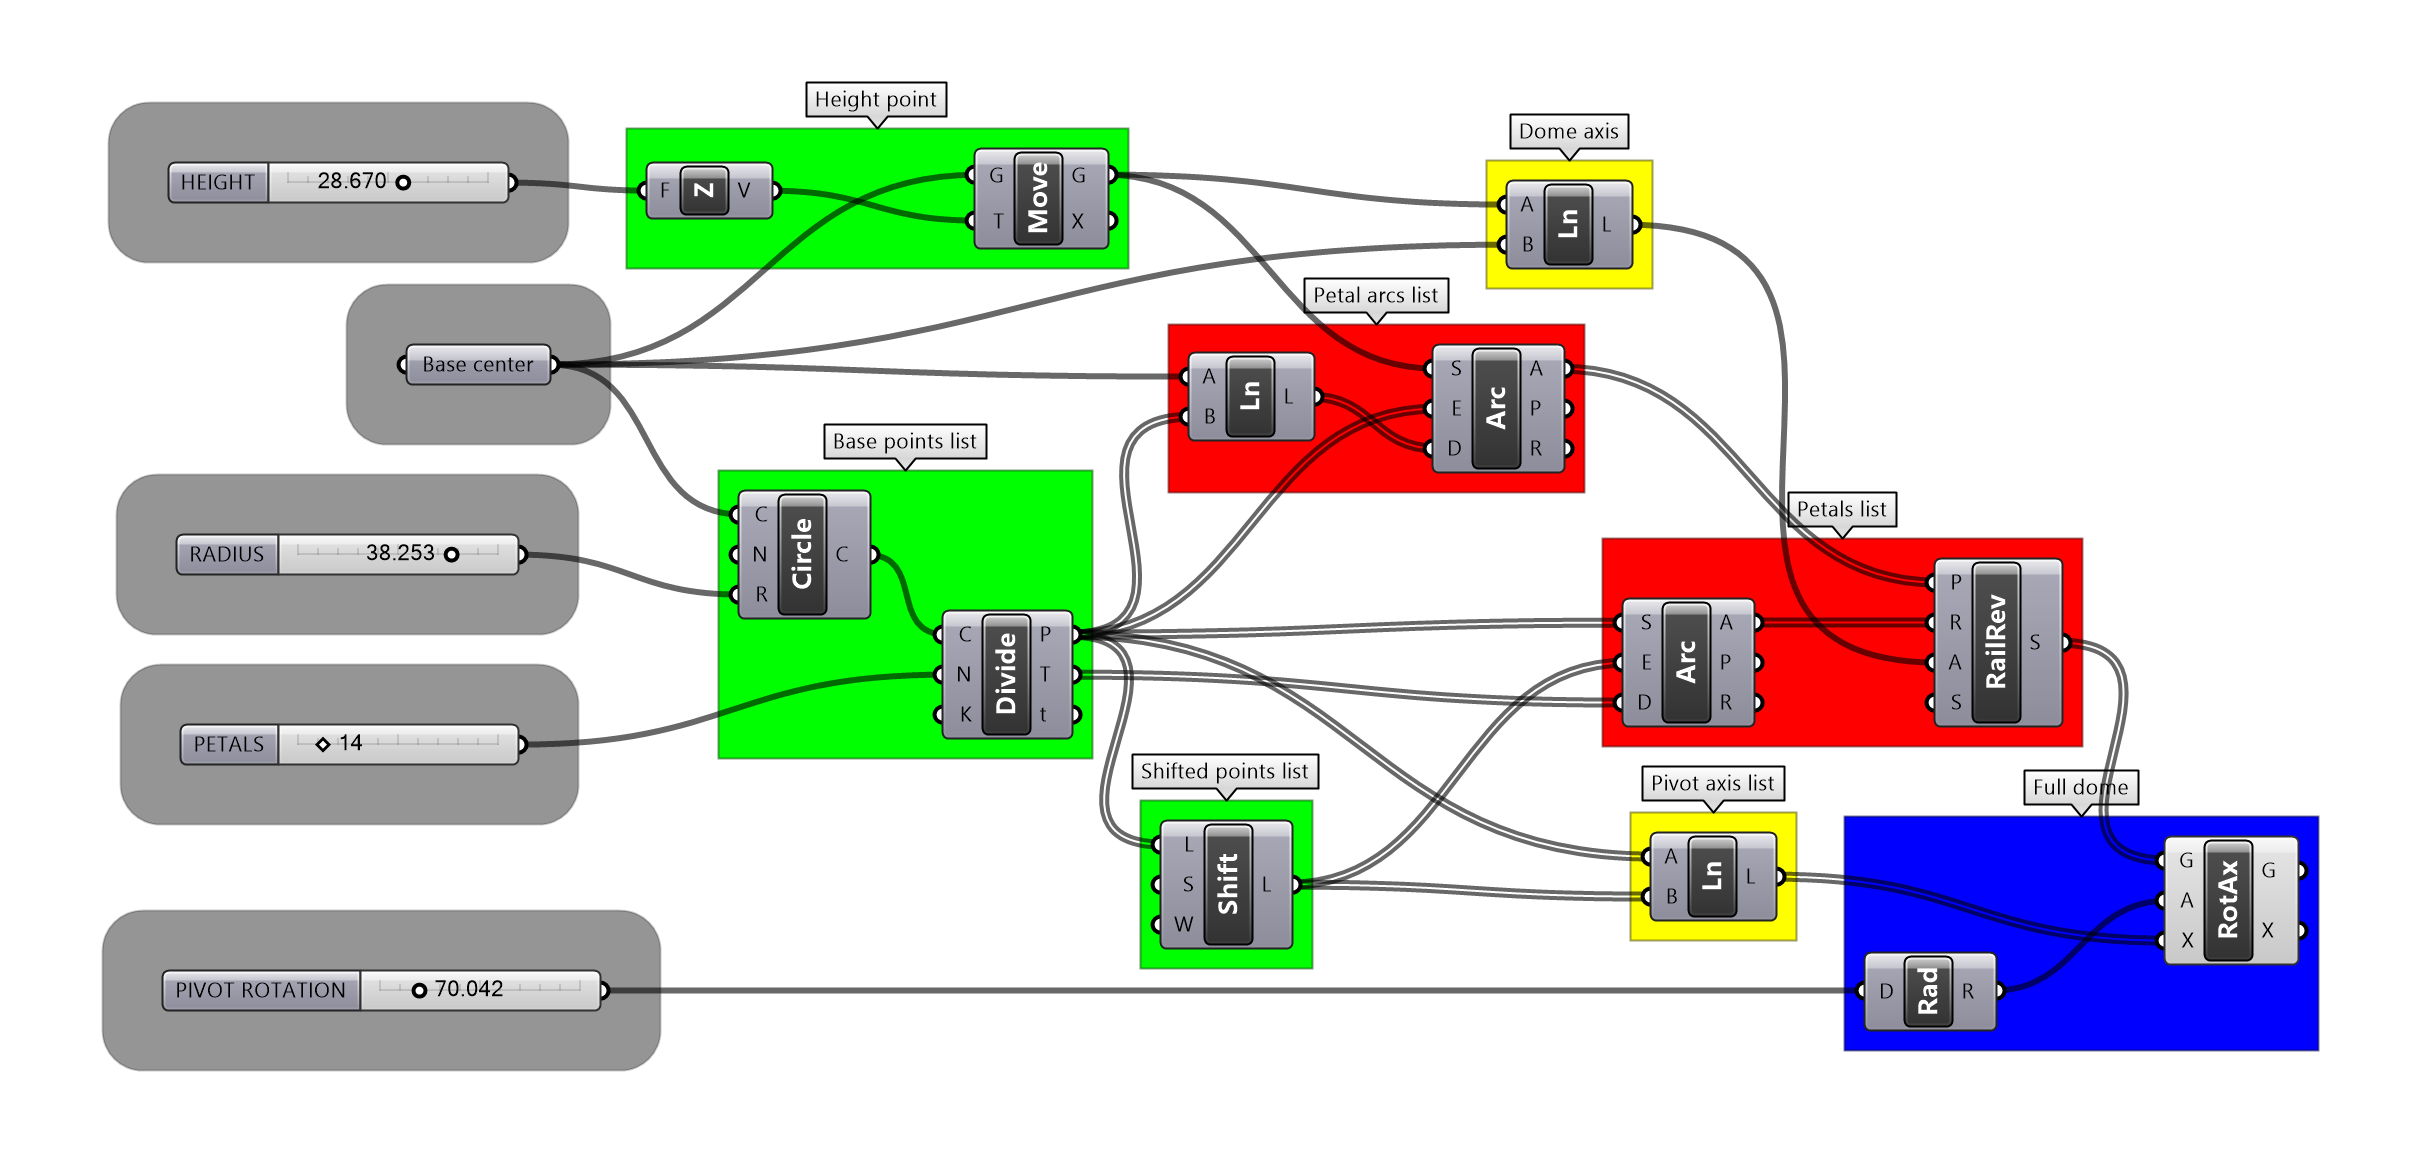
\includegraphics[width=0.95
\textwidth]{alg02.png}
\caption{List manipulation-based algorithm}
\label{figura:alg02}
\end{center}
\end{figure}

Until this point, we have used the ordered lists to execute commands that operate on elements of the lists, and no explicit manipulation has been required. A simple but important operation on the \textbf{base points list} is part of the proposed rules, and is used to generate the forms and exemplify the applications of this programming methodology. The idea is to extract the first element of a list, and append it to the end of the list. In the proposed points list represented as $A, B, C, D$ and $E$, this operation outputs $B, C, D, E$ and $A$. Generating lines between equivalent points in the two lists results in a list of lines that connects adjacent points: ($\bar{AB}, \bar{BC}, \bar{CD}$, and $\bar{DE}$). In Figure \ref{figura:alg02} this operation is represented in the bottom green box by taking the \textbf{base points list} (middle green box) and generating the \textbf{shifted points list}.

The \textbf{shifted points list} is directly used in the two steps of the algorithm. The first is used to create a \textbf{pivot axes list} by drawing lines between the \textbf{base points list} and the \textbf{shifted points list} (Fig. \ref{figura:alg02} bottom yellow box). The second is used to generate auxiliary arcs on the \textbf{petal surface list} creation (Fig. \ref{figura:alg02} bottom red box). The middle green box in Figure \ref{figura:alg02} generates the \textbf{base points list} by dividing the \textbf{base circle} by the given \textbf{number of petals}. The Grasshopper curve division component also generates a list of the tangent vectors of the curve at the division points. Arcs are drawn with a start point provided by the \textbf{base points list}, end points defined by the correspondent elements in the \textbf{shifted points list}, and with the sense and directions of the equivalent tangent vectors. These auxiliary arcs are used in place of the \textbf{petal angle} in the first algorithm to define the magnitude of the revolution angle of the petal surface (Fig. \ref{figura:alg02} bottom red box) around the \textbf{dome axis} (Fig. \ref{figura:alg02} top yellow box). Depending on the programming environment in which the code is implemented, the strategy of using auxiliary arcs or the one that calculates the \textbf{petal angle}, presented in Section \ref{geometric}, could be considered more suitable to generate the petals' surface, but both produce the same results.

The petal surface list (Fig. \ref{fig:a02s08}) is rotated around the correspondent \textbf{pivot axes list} by the angle provided by the pivot rotation parameter, hence drawing the \textbf{full dome} (Fig. \ref{fig:a02s09}).

\section{Analyzing the algorithm outputs}
\label{outs01}

\begin{figure}[h]
\begin{subfigure}{0.3\textwidth}
  \centering
  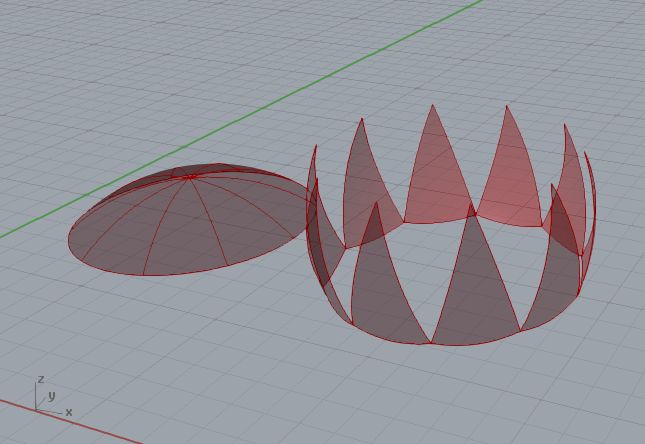
\includegraphics[width=.9\linewidth]{dome01.png}
  \caption{}
  \label{fig:dome01}
\end{subfigure}%
\begin{subfigure}{0.3\textwidth}
  \centering
  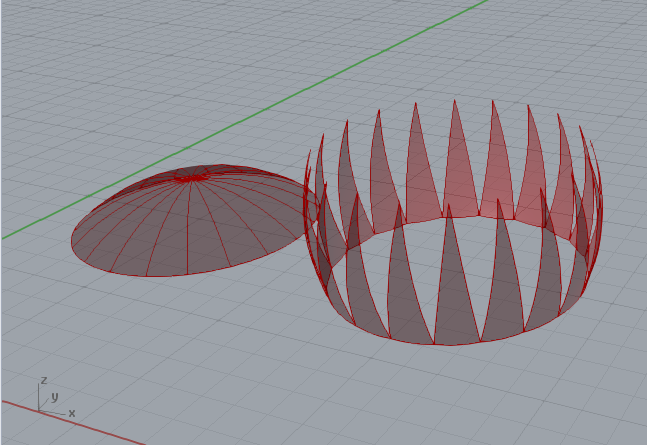
\includegraphics[width=.9\linewidth]{dome02.png}
  \caption{}
  \label{fig:dome02}
\end{subfigure}
\begin{subfigure}{0.3\textwidth}
  \centering
  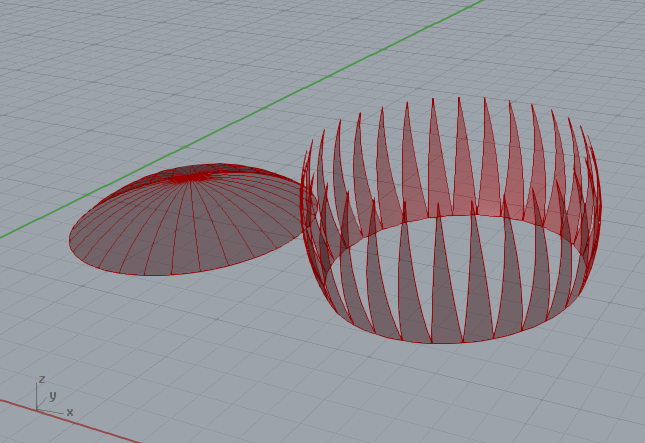
\includegraphics[width=.9\linewidth]{dome03.png}
  \caption{}
  \label{fig:dome03}
\end{subfigure}


\begin{subfigure}{0.3\textwidth}
  \centering
  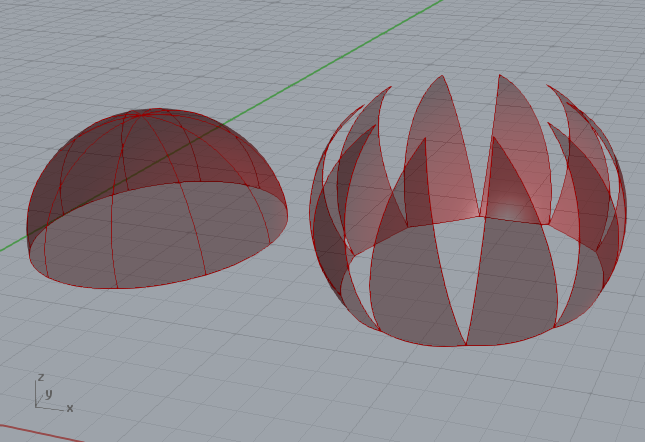
\includegraphics[width=.9\linewidth]{dome04.png}
  \caption{}
  \label{fig:dome04}
\end{subfigure}
\begin{subfigure}{0.3\textwidth}
  \centering
  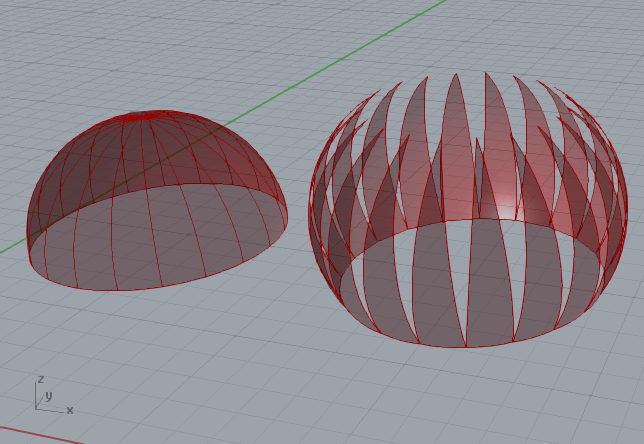
\includegraphics[width=.9\linewidth]{dome05.png}
  \caption{}
  \label{fig:dome05}
\end{subfigure}
\begin{subfigure}{0.3\textwidth}
  \centering
  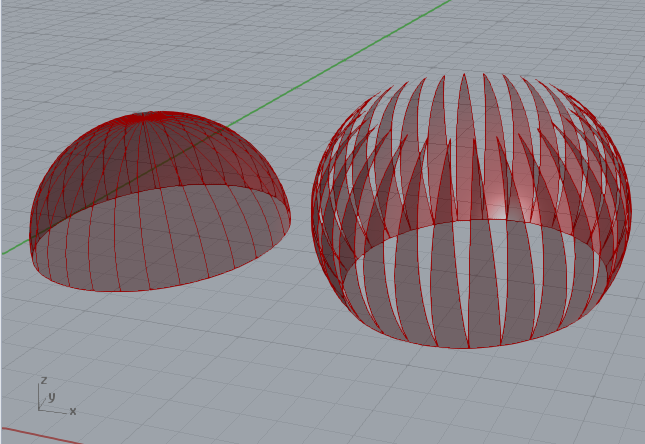
\includegraphics[width=.9\linewidth]{dome06.png}
  \caption{}
  \label{fig:dome06}
\end{subfigure}


\begin{subfigure}{0.3\textwidth}
  \centering
  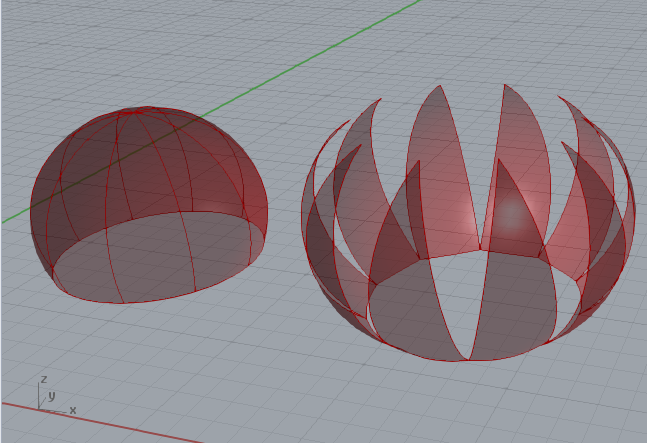
\includegraphics[width=.9\linewidth]{dome07.png}
  \caption{}
  \label{fig:dome07}
\end{subfigure}
\begin{subfigure}{0.3\textwidth}
  \centering
  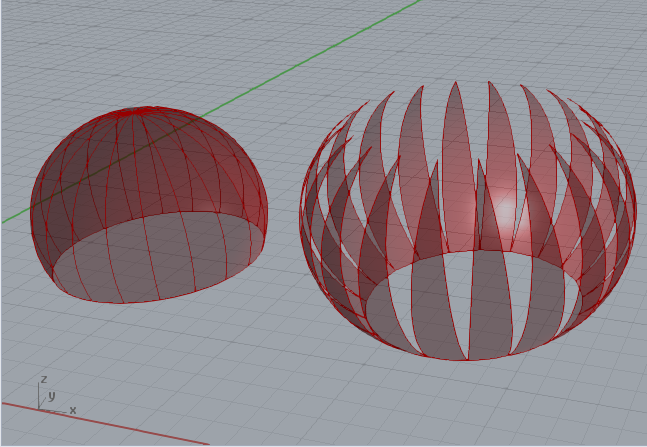
\includegraphics[width=.9\linewidth]{dome08.png}
  \caption{}
  \label{fig:dome08}
\end{subfigure}
\begin{subfigure}{0.3\textwidth}
  \centering
  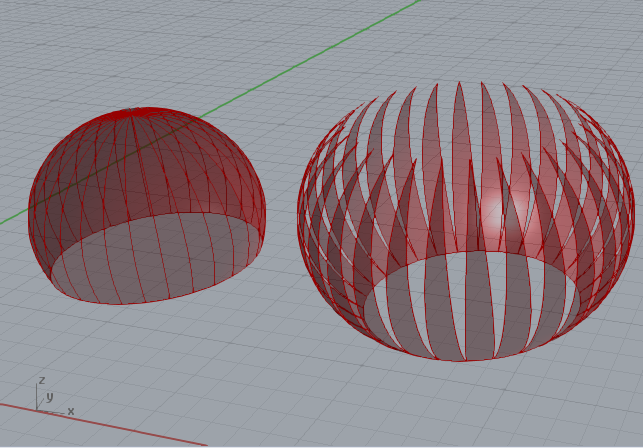
\includegraphics[width=.9\linewidth]{dome09.png}
  \caption{}
  \label{fig:dome09}
\end{subfigure}


\caption{Variant domes created by the algorithms}
\label{fig:domeresult}
\end{figure}

The flowchart in Figure \ref{figura:fluxogramametodologia} shows the scenario where, once the idea is established, the rules are planned, the code is implemented, and a form is generated by the first set of parameters, the designer is in charge of evaluating the result, resetting the parameters, and/or modifying the code, and continually repeats this proceedings until a constructive form is selected as the one to be built.

Figure \ref{fig:domeresult} shows a set of solutions generated exclusively by modifications made over the values of the parameters. One of the decisions that the designer should make is the size of the \textbf{base radius}, which is strongly related to the amount of light and the dynamics of the air that should circulate in and out of the building. This evaluation can depend on the designer's experience, and intuition or calculations that can be performed without the aid of computational analysis tools. Since the variations of forms are automatically generated, a tool that analyzes 3D models tends to be more efficient for the task.

Not only the building itself, but the characteristics of the environment should be considered in this choosing process. However, some relations between the parameters result in relevant changes in the generated geometries. In the first row of Figure \ref{fig:domeresult}, the domes have larger values for the \textbf{base radius} than for the \textbf{height} parameter; the second line shows equal values, and in the third row, the \textbf{radius} is smaller than the \textbf{height}. This fact can be easily demonstrated geometrically. 

The aesthetic impression made by the different simulations can be observed in the images of Figure \ref{fig:domeresult}, but is better understood when compared to the domes and respective buildings of Figures \ref{figura:sarah} and \ref{figura:trt}. The first one represents a larger value for the \textbf{height} parameter than the \textbf{radius}, producing a fluid relation between the curves of the building's forms and the dome as a finishing element. An inverted configuration of parameters in the relations between these values generates a brusque or even flat interruption of the composition of the forms. In the second figure, the domes adopt a more discrete elevation from the base, dialogging with the almost-flat roof solution of the buildings.

While the quantitative investigations can be numerically evaluated, the qualitative aspects, as aesthetics, can only be approached and addressed by the raising and answering of some loosely defined questions. The simple analysis proposed here aims to exemplify how these subjective questions can be handled by the methodology of generative algorithms.


\section{Modifying the code}
\label{extrap}

\begin{figure}[h]
\begin{subfigure}{0.3\textwidth}
  \centering
  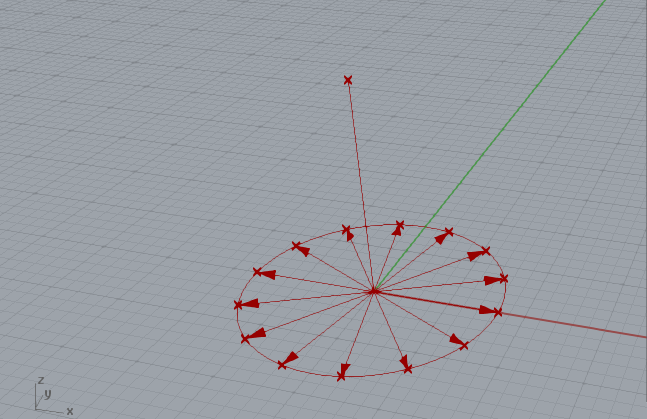
\includegraphics[width=.9\linewidth]{ag03s01.png}
  \caption{Auxiliary vectors list}
  \label{fig:ag03s01}
\end{subfigure}%
\begin{subfigure}{0.3\textwidth}
  \centering
  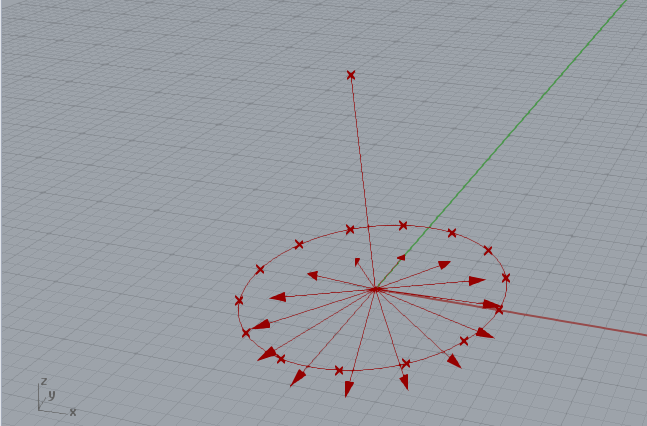
\includegraphics[width=.9\linewidth]{ag03s02.png}
  \caption{Rotated tangents list}
  \label{fig:ag03s02}
\end{subfigure}
\begin{subfigure}{0.3\textwidth}
  \centering
  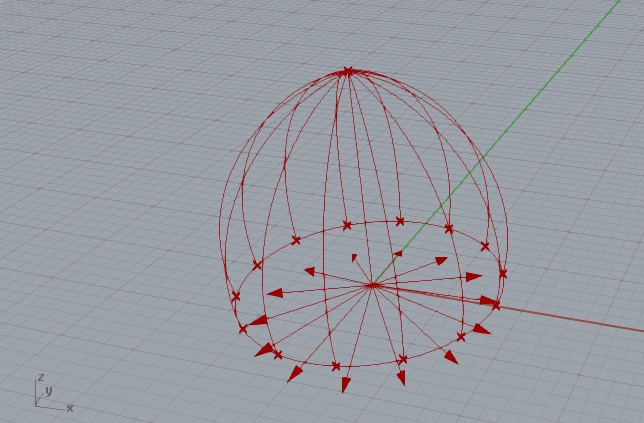
\includegraphics[width=.9\linewidth]{ag03s03.png}
  \caption{Petals arcs lists}
  \label{fig:ag03s03}
\end{subfigure}

\caption{Steps of the lancet dome algorithm}
\label{fig:lancetdome}
\end{figure}

Modification of the parameters is the fastest way to generate alternative results in a generative design system. The results registered in Figure \ref{fig:domeresult} can be generated by both the algorithms presented, but the flowchart in Figure \ref{figura:fluxogramametodologia} foresees that the code and the rules can also be modified within the scope of the methodology proposed here. To illustrate this possibility, some changes in the list manipulation-based algorithm are proposed to enable the code to create not only spherical cap domes, but also geometries derived from lancet arcs.

A few modifications are needed to complete this task. The steps presented in Figure \ref{fig:a02steps} are followed in exact order until the \textbf{auxiliary vectors} are created (Fig. \ref{fig:a02s06}). Then, the vectors undergo a rotation defined by a new parameter called \textbf{tangent rotation}, and the \textbf{petals arcs list} is created by taking these new vectors as inputs. Following this,\textbf{ the petal surface} list and the \textbf{full dome} are created by the same procedures as shown in Figures \ref{fig:a02s08} and \ref{fig:a02s09}.



\begin{figure}[h]
\begin{subfigure}{0.3\textwidth}
  \centering
  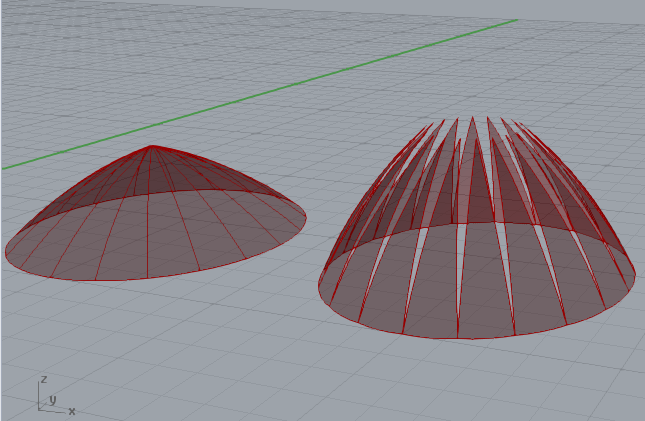
\includegraphics[width=.9\linewidth]{lancetDome01.png}
  \caption{}
  \label{fig:lancetDome01}
\end{subfigure}%
\begin{subfigure}{0.3\textwidth}
  \centering
  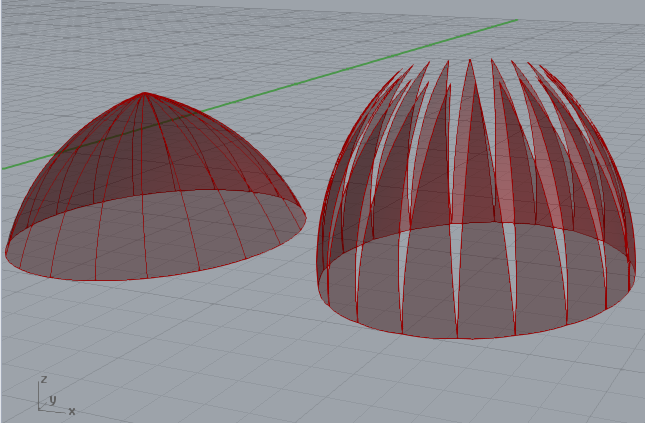
\includegraphics[width=.9\linewidth]{lancetDome02.png}
  \caption{}
  \label{fig:lancetDome02}
\end{subfigure}
\begin{subfigure}{0.3\textwidth}
  \centering
  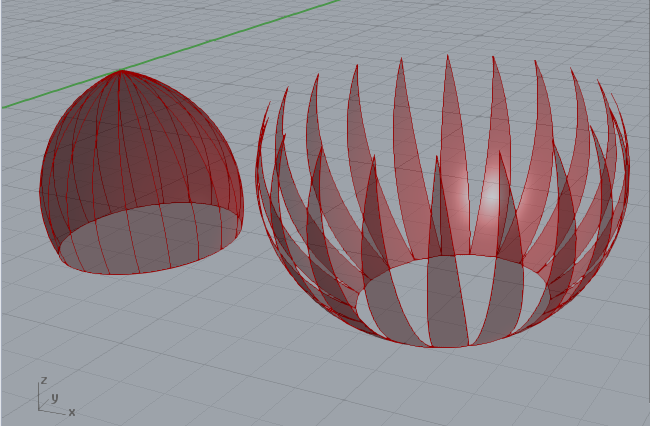
\includegraphics[width=.9\linewidth]{lancetDome03.png}
  \caption{}
  \label{fig:lancetDome03}
\end{subfigure}

\caption{Variant domes created by the lancet arcs algorithm}
\label{fig:lancetdomeexamples}
\end{figure}

If the tangent rotation parameter is equal to zero, the results are constrained to geometries similar to the ones presented in Figure \ref{fig:domeresult}; otherwise, they assume the pointed end of a lancet arc, as Figure \ref{fig:lancetdomeexamples} illustrates.

\begin{figure}[!h]
\begin{center}
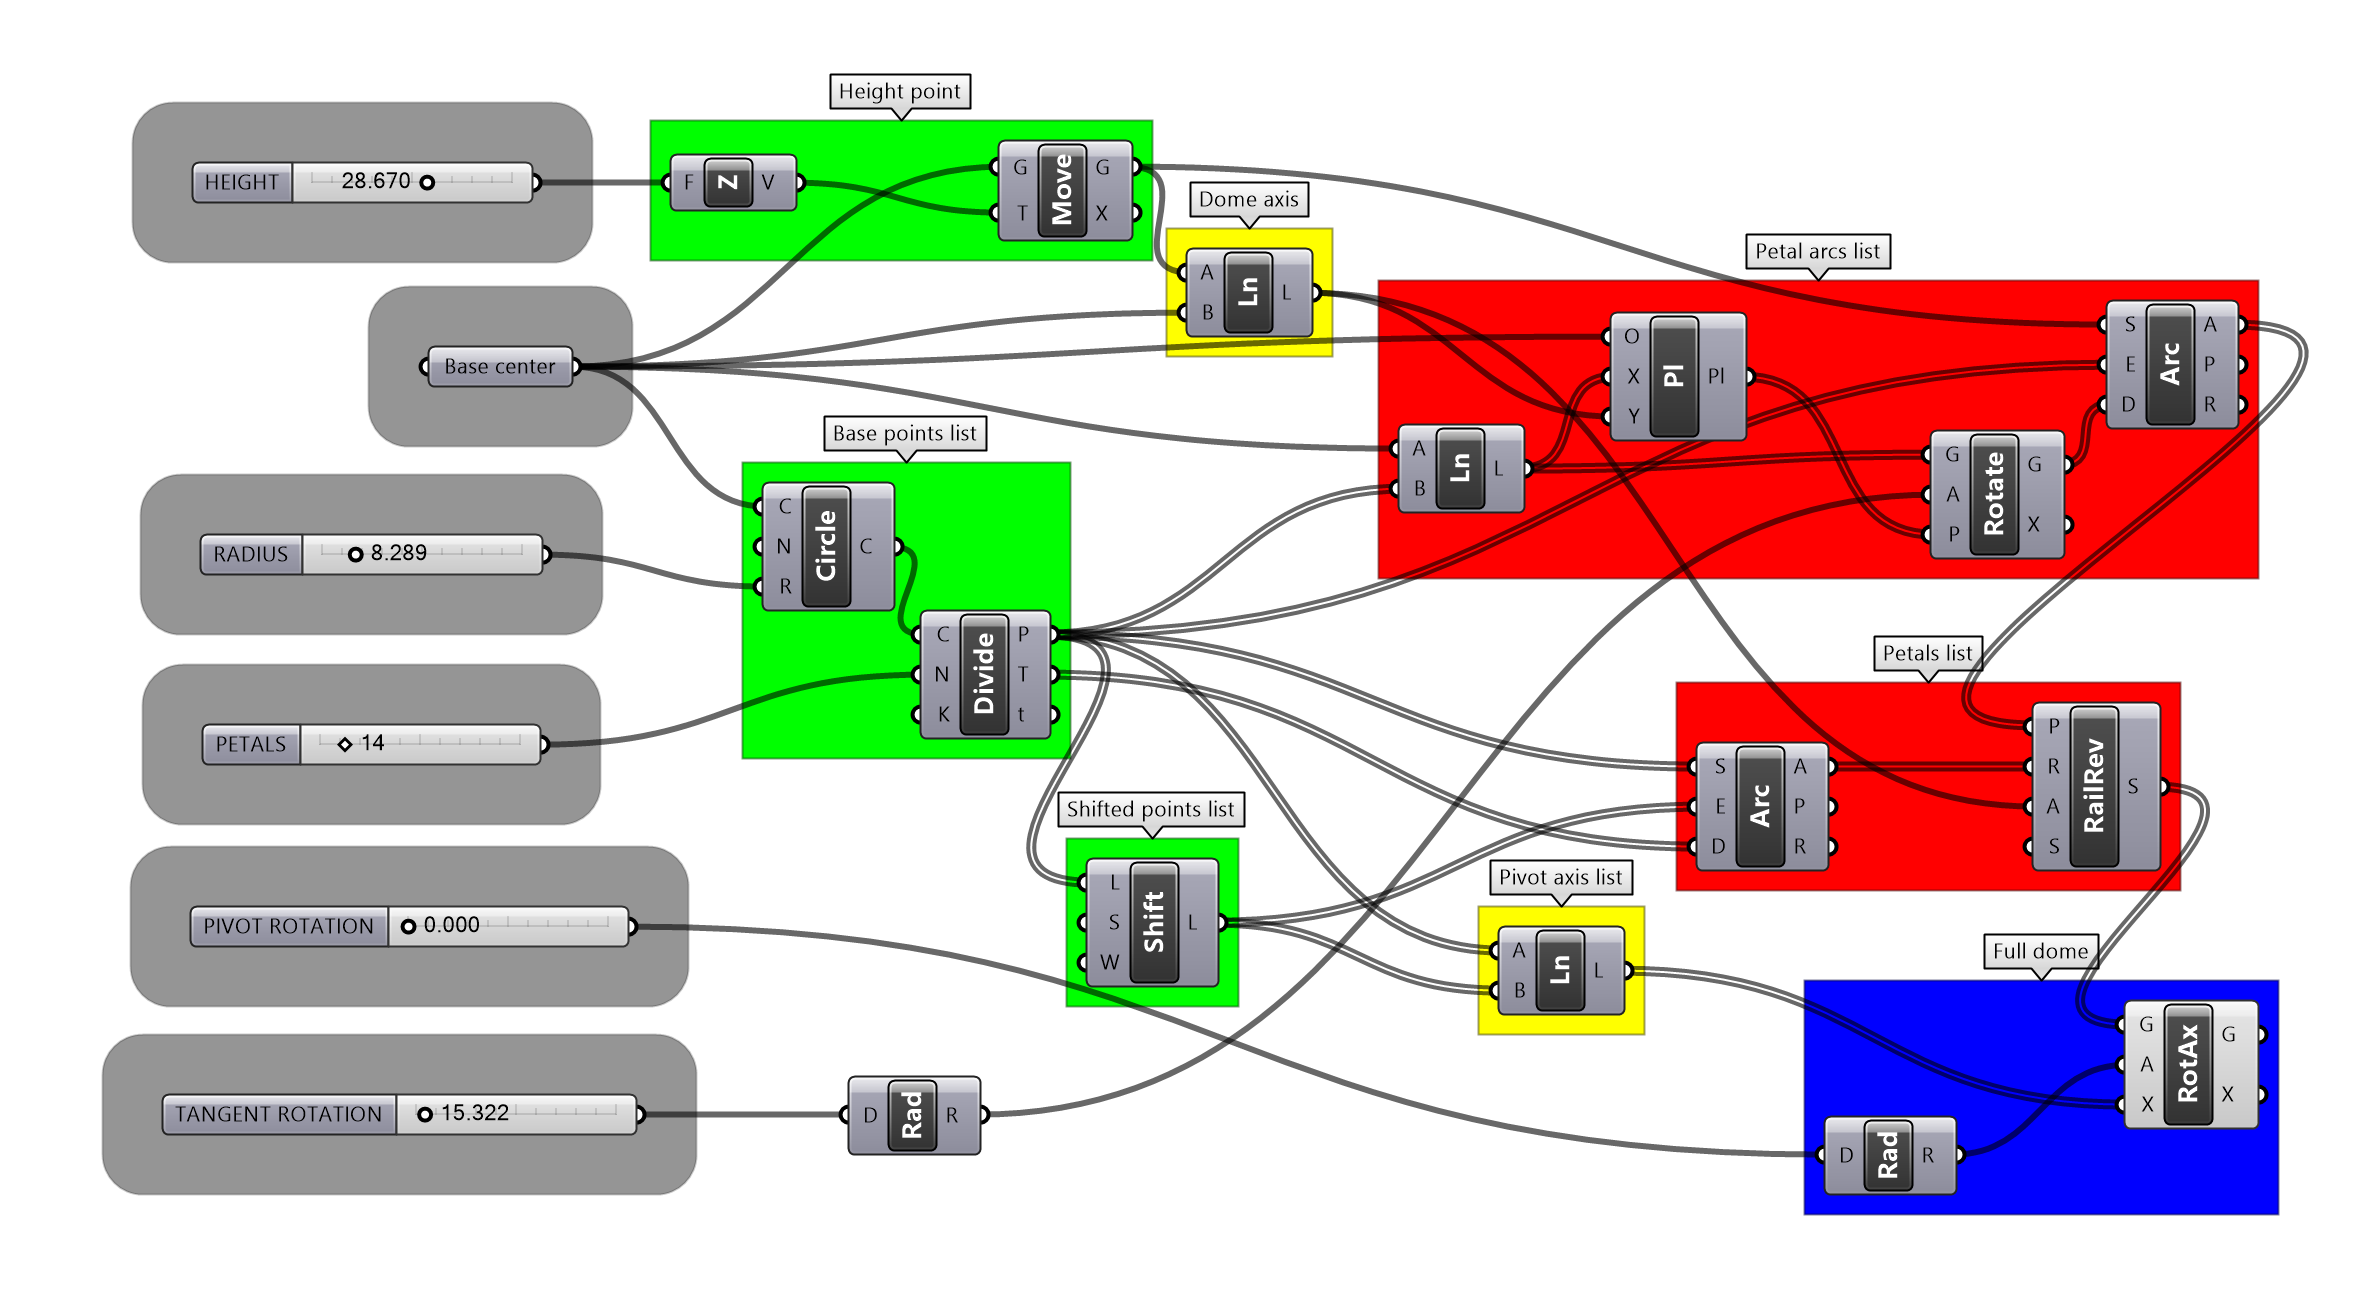
\includegraphics[width=0.95
\textwidth]{alg03.png}
\caption{Lancet arc algorithm}
\label{figura:alg03}
\end{center}
\end{figure}

The visual code presented in Figure \ref{figura:alg03} shows these changes in comparison with Figure \ref{figura:alg02}. The \textbf{tangent rotation} parameter is added (bottom grey box), and the \textbf{auxiliary vectors} are rotated around the $z$-axes of a list of planes created with origin at the \textbf{base center}. The $x$-axes are rotated in the direction and sense of the \textbf{auxiliary vectors}, and the $y$-axes follow the \textbf{dome axis}-oriented line. This rotated tangents' list is entered as the vector required by the \textbf{petal arcs list} creation component (top red box). 


\section{Conclusion}
\label{conc}

The proposed exercise discussed in this article succeeded in approaching the basics aspects of the generative design methodology, encompassing all possible variants of the flowchart in Figure \ref{figura:fluxogramametodologia}, explaining the most important geometric constructions used, providing an overview of some programming procedures, and presenting the manner in which constructive forms can be chosen from both qualitative and quantitative aspects.

The one-sentence definition of the idea purposely omits the fact that in the stage of analysis of the domes' references, they are all spherical caps. If this were stated, the modification to the algorithm in Section \ref{extrap} would also have modified the idea. Although this modification is not described in the flowchart (Fig. \ref{figura:fluxogramametodologia}), it is a possible move in the process of a generative algorithm. Since code reuse is a common programming activity, the case of the stated characteristic of an idea being modified along these lines should not be treated as an issue, but as a natural possibility. 

A comprehensive understanding of generative design systems demands an interdisciplinary perspective along with the interdisciplinary nature of architecture. The scope of all the different disciplines involved in this exercise was not comprehensively covered by any means, but the effort of bringing these ideas together in a coherent context should guide future work in the area.


%\appendix

%\section{Implemented test algorithms}
%\label{appendix-sec1}



%% References
%%
%% Following citation commands can be used in the body text:
%% Usage of \cite is as follows:
%%   \cite{key}         ==>>  [#]
%%   \cite[chap. 2]{key} ==>> [#, chap. 2]
%%

%% References with bibTeX database:

\bibliographystyle{elsarticle-num}
% \bibliographystyle{elsarticle-harv}
% \bibliographystyle{elsarticle-num-names}
% \bibliographystyle{model1a-num-names}
% \bibliographystyle{model1b-num-names}
% \bibliographystyle{model1c-num-names}
% \bibliographystyle{model1-num-names}
% \bibliographystyle{model2-names}
% \bibliographystyle{model3a-num-names}
% \bibliographystyle{model3-num-names}
% \bibliographystyle{model4-names}
% \bibliographystyle{model5-names}
% \bibliographystyle{model6-num-names}

\bibliography{library}


\end{document}

%%
%% End of file `elsarticle-template-num.tex'.

